\documentclass[12pt, a4paper]{article}

\usepackage[utf8]{inputenc}
\usepackage[framemethod=TikZ]{mdframed}
\usepackage[hidelinks]{hyperref}
\usepackage{mathtools, amssymb, amsmath, cleveref, fancyhdr, geometry, tcolorbox, graphicx, float, subfigure, arydshln, url, setspace, framed, pifont, physics, ntheorem, utopia}
%%% for coding %%%
\usepackage{listings}
\usepackage[ruled, vlined, linesnumbered]{algorithm2e}

\geometry{a4paper, left=2cm, right=2cm, bottom=2cm, top=2cm}

\pagestyle{fancy}
\fancyhead{}
\fancyhead[L]{\leftmark}
\fancyhead[R]{\rightmark}
\fancyfoot{}
\fancyfoot[C]{\thepage}
%\renewcommand{\headrulewidth}{0pt}
\renewcommand{\footrulewidth}{0pt}

\hypersetup{
	colorlinks = true,
	bookmarks = true,
	bookmarksnumbered = true,
	pdfborder = 001,
	linkcolor = blue
}


\newcounter{index}[subsection]
\setcounter{index}{0}
\newenvironment*{df}[1]{\par\noindent\textbf{Definition \thesubsection.\stepcounter{index}\theindex\ (#1).}}{\par}

\newenvironment*{eg}{\begin{framed}\par\noindent\textbf{Example \thesubsection.\stepcounter{index}\theindex}}{\par\end{framed}}

\newenvironment*{thm}[1]{\begin{tcolorbox}\par\noindent\textbf{Theorem \thesubsection.\stepcounter{index}\theindex\ #1} \par}{\par\end{tcolorbox}}

\newenvironment*{cor}[1]{\par\noindent\textbf{Corollary \thesubsection.\stepcounter{index}\theindex\ (#1).}}{\par}
\newenvironment*{lem}[1]{\par\noindent\textbf{Lemma \thesubsection.\stepcounter{index}\theindex\ (#1).}}{\par}
\newenvironment*{ax}[1]{\par\noindent\textbf{Axiom \thesubsection.\stepcounter{index}\theindex\ (#1).}}{\par}
\newenvironment*{prop}[1]{\par\noindent\textbf{Proposition \thesubsection.\stepcounter{index}\theindex\ (#1).}}{\par}
\newenvironment*{conj}[1]{\par\noindent\textbf{Conjecture \thesubsection.\stepcounter{index}\theindex\ (#1).}}{\par}
\newenvironment*{nota}{\par\noindent\textbf{Notation \thesubsection.\stepcounter{index}\theindex.}}{\par}

\newcounter{nprf}[subsection]
\setcounter{nprf}{0}
\newenvironment*{prf}{\par\indent\textbf{\textit{Proof \stepcounter{nprf}\thenprf.}}}{\hfill$\blacksquare$\par}
\newenvironment*{dis}{\par\indent\textbf{\textit{Disproof \stepcounter{nprf}\thenprf.}}}{\hfill$\blacksquare$\par}
\newenvironment*{sol}{\par\indent\textbf{\textit{Solution \stepcounter{nprf}\thenprf.}}\par}{\hfill{$\square$}\par}

\newtheorem*{hint}{Hint.}
\newtheorem*{rmk}{Remark.}
\newtheorem*{ext}{Extension.}

\linespread{1.2}

\title{Emory University\\\textbf{MATH 212 Differential Equations Learning Notes}}
\author{Jiuru Lyu}
\date{\today}

\def\Z{{\mathbb{Z}}}
\def\R{{\mathbb{R}}}
\def\C{{\mathbb{C}}}
\def\Q{{\mathbb{Q}}}
\def\E{{\mathbb{E}}}
\def\d{{\mathrm{d}}}
\def\i{{\mathrm{i}}}
\def\Arg{{\mathrm{Arg}}}
\def\cis{\mathrm{cis}}
\def\epsilon{\varepsilon}
\def\phi{\varphi}
\def\emptyset{\varemptyset}
\def\dsst{\displaystyle}
\def\pqde{\quad\square}
\def\A{\vb A}
\def\Y{\vb Y}

\begin{document}
\maketitle

\tableofcontents

\newpage
\section{First Order ODEs}
\subsection{Introduction}
\begin{df}{Ordinary Differential Equations/ODEs}
	An \textit{ordinary differential equation} is an equation that contains one or more derivatives of an unknown function $y=y(x)$.
\end{df}
\begin{df}{Order of ODEs}
	The \textit{order} of an ODE is the maximum order of the derivatives appearing in the equation.
\end{df}
\begin{df}{Solution to ODEs}
	The \textit{solution} to an ODE is a function $y$ that satisfies the equation.	
\end{df}
\begin{eg}
	Solve $y''=3x+1$.
	\begin{sol}
		\[\begin{aligned}y'&=\int3x+1\ \d x=\dfrac{3}{2}x^2+x+C\\y&=\int y'\ \d x=\int\dfrac{3}{2}x^2+x+C\ \d x=\dfrac{1}{2}x^3+\dfrac{1}{x}x^2+Cx+D.\end{aligned}\]
	\end{sol}
\end{eg}
\begin{df}{Linear ODEs/Non-Linear ODEs}
	A first order ODE is \textit{linear} if it can be written as \[y'+p(x)y=f(x).\] Otherwise, it is \textit{non-linear}.
\end{df}
\begin{df}{Homogenous/Non-Homogenous Linear ODEs}
	If $f(x)=0$, then the linear ODE is \textit{homogenous}. That is, \[y'+p(x)y=0.\] Otherwise, it is \textit{non-homogenous}.
\end{df}
\begin{df}{Trivial/Non-Trivial Solution}
	$y=0$ is a \textit{trivial solution} to a homogenous ODE. Any other solutions are \textit{non-trivial}.	
\end{df}
\begin{df}{One-Parameter Family of Solutions}
	We call $C$ a \textit{parameter} and the equation, therefore solution, defines a \textit{one-parameter family} of solutions.	
\end{df}
\begin{eg}
	For the ODE $y'=1$, $y_1=x+C_1$ is a solution to it, and it is a one-parameter family of solutions. Similarly, for $y'=\dfrac{1}{x^2}$, the one-parameter families of solutions are defined by $y_2=-\dfrac{1}{x}+C_2$ on the interval $(-\infty,0)\cup(0,\infty)$.
\end{eg}
\begin{df}{General Solution}
	Given the general form of the linear ODE $y'+p(x)y=f(x)$ if $p$ and $f$ are continuous on some open interval $(a,b)$ and there is a unique formula $y=y(x,c)$ and we have the following properties: 
	\begin{itemize}
		\item for each fixed $c$, the resulting function of $x$ is a solution of the ODE on $(a,b)$, and
		\item if $y$ is a solution of the ODE, then $y$ can be obtained by choosing the value of $c$ appropriately. 
	\end{itemize}
	The function $y=y(x,c)$ is called a \textit{general solution}. \par More generally, we can write an ODE as \[P_0(x)y'+P_1(x)y=F(x).\] In this case, the ODE has a general solution on any open interval in which $P_0,\ P_1,$ and $F$ are continuous and $P_0\neq0$.
\end{df}
\begin{df}{Initial Value Problem (IVP)}
	A differential equation with an initial condition.
\end{df}
\begin{eg}
	Let $a$ be a constant. Find the general solution of $y'-ay=0$ and solve the IVP $\begin{cases}y'-ay=0\\y(x_0)=y_0.\end{cases}$
	\begin{sol}
		Classification: First order, Linear, Homogeneous.\par Trivial Solution: $y=0$.\par General solution: \[\begin{aligned}\dv{y}{x}&=ay\\\int\dfrac{1}{y}\ \d y&=\int a\ \d x\\\ln\qty|y|&=ax+c\\y&=e^{ax+c}=Ae^{ax}.\end{aligned}\]\par\textit{This general solution includes the trivial solution.}\par IVP: Substitute $x=x_0$ and $y=y_0$: \[y_0=Ae^{ax_0}\quad\longrightarrow\quad A=y_0e^{-ax_0}\]\par So, \[y^\text{IVP}=y_0e^{-ax_0}e^{ax}=y_0e^{a(x-x_0)}.\]\par \textit{This IVP is a ``generic initial condition.'' We need more information on $x_0, y_0$ to get a more specific solution. }
	\end{sol}
\end{eg}

\subsection{Linear First Order ODEs}
\begin{thm}{}
	If $p$ is continuous on $(a,b)$, then the general solution of the homogeneous equation $y'+p(x)y=0$ on $(a,b)$ is given by \[y=ce^{-\int p(x)\ \d x}.\]
\end{thm}
\begin{prf}\par 
	(a). Substitute the solution formula to show that $y=ce^{-\int p(x)\ \d x}$ is a solution for any choice of $c$. \[y'=c\qty(-\int p(x)\ \d x)'e^{-\int p(x)\ \d x}=-cp(x)e^{-\int p(x)\ \d x}.\] Then, \[y'+p(x)y=-cp(x)e^{-\int p(x)\ \d x}+cp(x)e^{-\int p(x)\ \d x}=0.\] So, $y=ce^{-\int p(x)\ \d x}$ is a solution for any choice of $c$. $\pqde$\par
	(b). Want to show: any solution of $y'+p(x)y=0$ can be written as $y=ce^{-\int p(x)\ \d x}$. Note that $y=0$ is a trivial solution, so we assume $y\neq0$. \[\begin{aligned}y'+p(x)y&=0\\y'&=-p(x)y\\\dfrac{y'}{y}&=-p(x)\\\leadsto\int\dfrac{1}{y}\ \d y&=\int-p(x)\ \d x\\\ln\qty|y|&=-\int p(x)\ \d x\\y&=ce^{-\int p(x)\ \d x}.\end{aligned}\] Note that when $c=0$, $y=0$ is the trivial solution. So, any solution of $y'+p(x)y=0$ can be written as $y=ce^{-\int p(x)\ \d x}$.
\end{prf}
\begin{eg}
	Solve the IVP \[\begin{cases}xy'+y=0\\y(1)=3.\end{cases}\]
	\begin{sol}
		Note that $P_0(x)=x$ and $P_1(x)=1$, which are continuous on $\R$. Since we need $P_0(x)\neq0$, $x\neq0$. So the interval of validity is $\R\backslash\qty{0}$.\par 
		$\boxed{\text{Method 1: Separation of Variables}}$ \[y'=-\dfrac{y}{x}.\] Note that $y=0$ is a solution. Assume $y\neq0$. \[\begin{aligned}\dfrac{y'}{y}=-\dfrac{1}{x}\quad\leadsto\quad\int\dfrac{1}{y}\ \d y&=-\int\dfrac{1}{x}\ \d x+k\\\ln\qty|y|&=-\ln\qty|x|+k\\\qty|y|&=e^{k}\dfrac{1}{\qty|x|}\\y&=\dfrac{c}{x}\end{aligned}\]\par 
		$\boxed{\text{Method 2: Solution Formula}}$ By Theorem 1.2.1, \[y=ce^{-\int p(x)\ \d x}=ce^{-\int\frac{1}{x}\ \d x}=ce^{-\ln\qty|x|}=\dfrac{c}{x}.\]\par 
		$\boxed{\text{Solving the IVP}}$ Substitute $x=1$ and $y=3$: \[3=\dfrac{c}{1}\quad\longrightarrow\quad c=3.\] So, $y^\text{IVP}=\dfrac{3}{x}$.
	\end{sol}
\end{eg}
\begin{eg}
	Given the equation $(4+x^2)y'+2xy=4x$. Classify the equation and find the general solution $y=y(x,c)$.
	\begin{sol}
		This is a first order, linear, non-homogeneous differential equation.\par
		Note that $P_0(x)=4+x^2$, $P_1(x)=2x$, $F(x)=4x$, and $P_0\neq0\ \forall x\in\R$, so the interval of validity is $\R$. Also note that $\dsst\dv{x}\qty\big[4+x^2]=2x$, so the equation can be written as \[(4+x^2)\dv{y}{x}+\dv{x}\qty\big[4+x^2]y=4x.\] Using the product rule to re-write the LHS as \[\begin{aligned}\dv{x}\qty\big[(4+x^2)y]&=4x\\\int\dv{x}\qty\big[(4+x^2)y]\ \d x&=\int 4x\ \d x+c\\(4+x^2)y&=2x^2+c\\y&=\dfrac{2x^2+c}{4+x^2}.\end{aligned}\]
	\end{sol}
\end{eg}
\begin{eg}
	Given the equation $y'-2y=4-x$. Classify the equation and find the general solution $y=y(x,c)$.
	\begin{sol}
		This is a first order, linear, non-homogeneous differential equation.\par
		Since $P_0(x)=1$, $P_1(x)=-2y$, $F(x)=4-x$, and $P_0(x)\neq0\ \forall x\in\R$, the interval of validity is $\R$. Consider $\mu=\mu(x)\neq0$. Multiply both sides of the equation by $\mu(x)$: \begin{equation}\label{eq1}\mu(x)y'-2\mu(x)y=\mu(x)(4-x)\end{equation} To make the LHS a product rule, we need \[\dv{x}\qty\big[\mu(x)y(x)]=\mu'(x)y(x)+\mu(x)y'(x)=\mu(x)y'(x)-2\mu(x)y.\] So, we have $\mu'=-2\mu$, or $\mu'+2\mu=0,$ a first order, linear, homogeneous ODE. Solving this ODE, we get $\mu(x)=ce^{-2x}$. Since we only want one specific $\mu$ that would work, take $c=1$. So, $\mu(x)=e^{-2x}$. Substituting $\mu(x)=e^{-2x}$ to Eq. (\ref{eq1}): \[e^{-2x}y'-2e^{-2x}y=e^{-2x}(4-x),\quad\widetilde{P}_0=e^{-2x}\neq0,\ \widetilde{P}_1=-2e^{-2x}.\] Using the product rule: \[\begin{aligned}\dv{x}\qty[e^{-2x}y]&=4e^{-2x}-xe^{-2x}\\\int\dv{x}\qty[e^{-2x}y]\ \d x&=\int 4e^{-2x}-xe^{-2x}\ \d x+c\\e^{-2x}y&=\dfrac{1}{2}xe^{-2x}-\dfrac{7}{4}e^{-2x}+c\\y&=e^{2x}\qty(\dfrac{1}{2}xe^{-2x}-\dfrac{7}{4}e^{-2x}+c)\\&=\dfrac{1}{2}x-\dfrac{7}{4}+ce^{2x}.\end{aligned}\]
	\end{sol}
\end{eg}
\begin{thm}{Method of Integrating Factor}
	Given the first order linear differential equation $y'+p(x)y=f(x)$, with $p$ and $f$ both continuous on some interval $(a,b)$, \[y(x)=\dfrac{1}{\mu(x)}\qty[\int\mu(x)f(x)\ \d x+c]\] is the general solution to the equation, with \[\mu(x)=e^{\int p(x)\ \d x}.\] We call $\mu(x)$ the \textit{integrating factor}.
\end{thm}
\begin{prf}
	Consider $\mu=\mu(x)\neq0$. Multiplying the both sides of $y'+p(x)y=f(x)$ by $\mu$: \begin{equation}\label{eq2}\mu y'+p\mu y=\mu f.\end{equation} Impose $\mu y'+p\mu y=\dsst\dv{x}\qty\big[\mu y]$ to find $\mu=\mu(x)$: \[\begin{aligned}\mu y'+p\mu y&=\mu' y+\mu y'\\\mu'-p\mu&=0,&\text{first order, linear, homogeneous ODE}\\\mu(x)&=e^{\int p(x)\ \d x}, &\text{the integrating factor}\end{aligned}\] Substitute $\mu(x)=e^{\int p(x)\ \d x}$ into Eq. (\ref{eq2}): \[\begin{aligned}\dv{x}\qty\big[\mu y]&=\mu f\\\int\dv{x}\qty\big[\mu y]\ \d x&=\int\mu f\ \d x+c\\\mu y&=\int\mu f\ \d x+c\\y(x)&=\dfrac{1}{\mu(x)}\qty[\int\mu(x)f(x)\ \d x+c].\end{aligned}\]
\end{prf}
\begin{eg}
	Give the equation $y'+2y=x^3e^{-2x}$. Classify the equation and find the general solution $y=y(x,c)$.
	\begin{sol}
		It is a first order, linear, non-homogeneous ODE, with $p=2$ and $f=x^3e^{-2x}$. Let $\mu(x)$ be the integrating factor. Then, \[\mu(x)=e^{\int2\ \d x}=e^{2x}.\] So, by the method of integrating factor, we know \[\begin{aligned}\dv{x}\qty\Big[\mu(x)y]&=\mu(x)f(x)\\\int\dv{x}\qty\Big[e^{2x}y]\ \d{x}&=\int e^{2x}x^3e^{-2x}\ \d{x}+c\\e^{2x}y&=\int x^3\ \d{x}+c\\e^{2x}y&=\dfrac{1}{4}x^4+c\\y&=\dfrac{1}{4}x^4e^{-2x}+ce^{-2x}.\end{aligned}\]
	\end{sol}
\end{eg}
\begin{rmk}
	Re-examine the formula we derived from the method of integrating factor: \[y(x)=\dfrac{1}{\mu}\int f\mu\ \d x+\boxed{\dfrac{c}{\mu}}.\] The part being boxed, $\dfrac{c}{\mu}$, is independent from $f$ and is exactly $ce^{-\int p\ \d x}$ if we expand, which is the solution for a homogeneous differential equation. 
\end{rmk}
\begin{df}{Complementary Equation}
	The \textit{complementary equation} to a first order ODE $y'+py=f$ is the homogeneous part of it. i.e., $y'+py=0$.	
\end{df}
\begin{thm}{Method of Variation of Parameters}
	Given the first order linear differential equation $y'+p(x)y=f(x)$, with $p$ and $f$ both continuous on some interval $(a,b)$, \[y(x)=y_1(x)\qty[\int\dfrac{f(x)}{y_1(x)}\ \d x+c]\] is the general solution to the equation, where $y_1$ is a solution of the complementary euqation $y'+py=0$.
\end{thm}
\begin{prf}
	Call $y_1$ a solution of the complementary equation $y'+p(x)y=0$. Then, we want to find $y(x)=u(x)y_1(x)$, the general solution of $y'+p(x)y=f(x)$, where $u$ is an unknown function of $f$. Note that, by product rule, $y'(x)=u'y_1+uy_1'$. Then, the equation becomes \[\begin{aligned}(u'y_1+uy_1')+p(x)(uy_1)&=f(x)\\u'y_1+uy_1'+puy_1&=f\\y_1u'+\underbrace{(y_1'+py_1)}_{0}u&=f\\y_1u'&=f\implies u(x)=\int\dfrac{f(x)}{y_1(x)}\ \d x+c.\end{aligned}\] Therefore, the formula to find $y$ is given by \[y=y_1u=y_1(x)\qty[\int\dfrac{f(x)}{y_1(x)}\ \d{x}+c].\]
\end{prf}
\begin{rmk}
	The method of variation of parameters will be more useful when solving second or higher order differential equations.	
\end{rmk}
\begin{eg}
	Give the equation $y'+2y=x^3e^{-2x}$. Find the general solution $y=y(x,c)$ using the method of variation of parameters.
	\begin{sol}
		It is a first order, linear, non-homogeneous ODE, with $p=2$ and $f=x^3e^{-2x}$. Let $y_1$ be the solution of the complementary equation $y'+2y=0$. Then, $y_1(x)=e^{-\int2\ \d{x}}=e^{-2x}$. By the method of variation of parameters, suppose $y=uy_1$, where $u$ is an unknown function of $x$. Then, \[u(x)=\int\dfrac{f(x)}{y_1(x)}\ \d{x}+c=\int\dfrac{x^3e^{-2x}}{e^{-2x}}\ \d{x}+c=\int x^3\ \d{x}+c=\dfrac{1}{4}x^4+c.\] So, \[y=uy_1=e^{-2x}\qty(\dfrac{1}{4}x^4+c)=\dfrac{1}{4}x^4e^{-2x}+ce^{-2x}.\]
	\end{sol}
\end{eg}
\begin{thm}{Existence and Uniqueness Theorem}
	Suppose that $p=p(x)$ and $f=f(x)$ are continuous on $(a,b)$. Then, a general solution of $y'+p(x)y=f(x)$ on $(a,b)$ is  \[y(x)=y_1(x)\qty[\int\dfrac{f(x)}{y_1(x)}\ \d{x}+c],\]	 where $y_1(x)$ is a solution of the complementary equation (i.e., $y'+p(x)y=0$).\par 
	If $x_0$ is an arbitrary point in $(a,b)$ and $y_0$ is an arbitrary real number, then the initial value problem, \[y'+p(x)y=f(x),\quad y(x_0)=y_0\] has a unique solution on $(a,b)$.
\end{thm}

\subsection{Separable Equations}
\begin{df}{General Forms}
	The general form of a non-linear first order ODE is given by \[y'=f\qty(x,y\qty(x)).\] If we take $M(x,y)=-f(x,y)$ and $N(x,y)=1$, we can also re-write the equation into \[M(x,y)+N(x,y)y'=0, \quad\text{or}\quad M(x,y)\ \d{x}+N(x,y)\ \d{y}=0.\]
\end{df}
\begin{df}{Separable Equations}
	If $M(x,y)=M(x)$ and $N(x,y)=N(y)$, then the ODE is called \textit{separable}.
\end{df}
\begin{thm}{Separation of Variables (SoV)}
	Consider the non-linear first order ODE $M(x,y)+N(x,y)y'=0$, with $M(x,y)=M(x)$ and $N(x,y)=N(y)$. Then we can find an implicit solution of the ODE in the form of \[F(x,y)=c,\] where $F(x,y)$ is a function of $x$ and $y$ and \[F(x,y)=\int M(x)\ \d{x}+\int N(y)\ \d{y}.\]
\end{thm}
\begin{prf}
	Let $H_1'(x)=M(x)$ and $H_2'(y)=N(y)$. Then, the equation becomes \[\begin{aligned}H_1'(x)+H_2'(y)y'&=0\\\dv{x}\qty\Big[H_1(x)]+\dv{y}\qty\Big[H_2(y)]\dv{y}{x}&=0\end{aligned}\] By using the chain rule, $\dsst\dv{y}\qty\Big[H_2(y)]\dv{y}{x}=\dv{x}\qty\Big[H_2\qty(y(x))].$ So, the equation becomes \[\begin{aligned}\dv{x}\qty\Big[H_1(x)]+\dv{x}\qty\Big[H_2\qty(y(x))]&=0\\\dv{x}\qty\Big[H_1(x)+H_2(y)]&=0\\H_1(x)+H_2(y)&=c\\\int M(x)\ \dv{x}+\int N(y)\ \d{y}&=c\\F(x,y)&=c\end{aligned}\]
\end{prf}
\begin{eg}
	Given the equation $\dsst y'=\dfrac{x^2}{1-y^2}$. Classify the differential equation and find the general solution.
	\begin{sol}
		It is a first order, non-linear ODE. Since $y'=\dfrac{x^2}{1-y^2}$, so we have $1-y^2\neq0$. That is, $y^2\neq1,$ or $y\neq\pm1$. Using the separation of variables (SoV), we have \[\begin{aligned}(1-y^2)y'&=x^2\\\int 1-y^2\ \d{y}&=\int x^2\ \d{x}\\y-\dfrac{1}{3}y^3&=\dfrac{1}{3}x^3+c\\y-\dfrac{1}{3}y^3-\dfrac{1}{3}x^3&=c\\3y-y^3-x^3&=c\end{aligned}\]
	\end{sol}
\end{eg}
\begin{eg}
	Given the equation $\dsst y'=\dfrac{(y-3)\cos{x}}{1+2y^2}$. Classify the equation and find the general solution.
	\begin{sol}
		It is a first order, non-linear ODE. Since $1+2y^2\neq0\quad\forall y\in\R$. Note that if we take $y-3=0$, we get $y=3$, a constant solution to the differential equation. Now, assume $y\neq3$. Then, use SoV: \[\int\dfrac{1+2y^2}{y-3}\ \d{y}=\int\cos{x}\ \d{x}+c=\sin{x}+c.\] Set $t=y-3$, $\d{t}=\d{y}$. So, $y=t+3$ and $y^2=(t+3)^2$. Then, \[\begin{aligned}\int\dfrac{1+2y^2}{y-3}\ \d{y}=\int\dfrac{1+2(t+3)^2}{t}\ \d{t}&=\int\dfrac{1+2t^2+12t+18}{t}\ \d{t}\\&=\int\dfrac{19}{t}+12+2t\ \d{t}\\&=19\ln\qty|t|+12t+t^2\\&=19\ln\qty|y-3|+12(y-3)+(y-3)^2\\&=19\ln\qty|y-3|+6y+y^2-27.\end{aligned}\] So, \[19\ln\qty|y-3|+y^2+6y-27-\sin{x}=c\]
	\end{sol}
\end{eg}
\begin{eg}
	Give the equation $y'=\dfrac{1}{2}x\qty(1-y^2)$. Classify the equation and find the general solution. 
	\begin{sol}
		It is a first order, non-linear ODE. Notice that we have the constant solutions when we take $1-y^2=0$, or $y=\pm1$. Now, assume $y\neq\pm1$. Using SoV: \[\int\dfrac{2}{1-y^2}\ \d{y}=\int x\ \d{x}+c=\dfrac{1}{2}x^2+c.\]	Note that $\dfrac{2}{1-y^2}=\dfrac{2}{(1-y)(1+y)}$. Use partial fractions. Assume \[\dfrac{2}{(1-y)(1+y)}=\dfrac{A}{1-y}+\dfrac{B}{1+y}.\] Then, we get $A(1+y)+B(1-y)=2$. That is, $(A+B)+(A-B)y=2$. Attempting to solve the system of equations $\begin{cases}A-B=0\\A+B=2\end{cases}$, then we get $A=B=1$.Therefore, \[\dfrac{2}{1-y^2}=\dfrac{1}{1-y}+\dfrac{1}{1+y}.\] Then, \[\begin{aligned}\int\dfrac{1}{1-y}+\dfrac{1}{1+y}\ \d{y}&=\dfrac{1}{2}x^2+c\\-\ln\qty|1-y|+\ln\qty|1+y|&=\dfrac{1}{2}x^2+c\\\ln\qty|1-y|-\ln\qty|1+y|&=-\dfrac{1}{2}x^2+c\\\ln\qty|\dfrac{1-y}{1+y}|&=-\dfrac{1}{2}x^2+c\\\qty|\dfrac{y-1}{y+1}|&=e^{-\frac{1}{2}x^2+c}=e^{-\frac{1}{2}x^2}e^c\\\dfrac{y-1}{y+1}&=c_2e^{-\frac{1}{2}x^2}\\y-1&=(y+1)c_2e^{-\frac{1}{2}x^2}\\(1-c_2e^{-\frac{1}{2}x^2})y&=1+c_2e^{-\frac{1}{2}x^2}\\y&=\dfrac{1+c_2e^{-\frac{1}{2}x^2}}{1-c_2e^{-\frac{1}{2}x^2}}\end{aligned}\] The value of $c_2$ si chosen according to the sign of $\dfrac{y-1}{y+1}.$
	\end{sol}
\end{eg}
\begin{eg}{}
	Given the equation $y'=\dfrac{3x^2+4x+2}{2(y-1)},$ with $y(0)=1$. Classify the equation, find the general solution, and solve the IVP. 
	\begin{sol}
		It is a first order, nonlinear, separable ODE. Note that $y-1\neq0$, so $y\neq1$. Assume $y\neq1,$ use SoV: \[\begin{aligned}\int2(y-1)\ \d{y}&=\int3x^2+4x+2\ \d{x}+c\\(y-1)^2&=x^3+2x^2+2x+c\\y^2-2y+1&=x^3+2x^2+2x+c\\y^2-2y&=x^3+2x^2+2x+c.\end{aligned}\] Substitute $y=-1$ when $x=0$: \[1+2=c\implies c=3.\] So, \[\begin{aligned}y^2-2y&=x^3+2x^2+2x+3,\quad y\neq1\\y^2-2y+1&=x^3+2x^2+2x+4\\(y-1)^2&=x^3+2x^2+2x+4\\y-1&=\pm\sqrt{x^3+2x^2+2x+4}\\ y&=1\pm\sqrt{x^3+2x^2+2x+4}.\end{aligned}\] If $y=-1$ and $x=0$: $-1=1\pm\sqrt{4}=1\pm2$. So, it must be that $-1=1-2$. So, \[y^\text{IVP}=1-\sqrt{x^3+2x^2+2x+4}.\] Note that now we have another condition for $x$: \[\begin{aligned}x^3+2x^2+2x+4&\geq0\\(x+2)(x^2+2)&\geq0\\x+2&\geq0\\x&\geq-2\end{aligned}\] So, \[y^\text{IVP}=1-\sqrt{x^3+2x^2+2x+4},\text{ with }y\neq1\text{ and }x\geq-2.\]
	\end{sol}
\end{eg}
\begin{eg}{}
	Solve the IVP $\begin{cases}y'=\sqrt[3]{y}=y^\frac{1}{3}\\y(0)=0\end{cases}$. 
	\begin{sol}
		It is a first order, nonlinear, separable ODE. The initial interval of validity: $x\in\R$ and $y\in\R$. Note that if $y=0$, there is a constant solution. Assume $y\neq0$, use $SoV$: \[\begin{aligned}\int y^{-\frac{1}{3}}\ \d{y}&=\int\ \d{x}+c\\\dfrac{3}{2}y^\frac{2}{3}&=x+c\\y^\frac{2}{3}&=\dfrac{2}{3}x+c\\y&=\pm\qty(\dfrac{2}{3}x+c)^\frac{3}{2}\end{aligned}\] Substitute $y(0)=0$: \[0=0+c\implies c=0.\] So, \[y^\text{IVP}=\pm\qty(\dfrac{2}{3}x)^\frac{3}{2}.\]
	\end{sol}
\end{eg}
\begin{thm}{Existence and Uniqueness of Solutions to Nonlinear ODEs}
	Consider the IVP \[y'=f(x,y(x))\quad\text{with }y(x_0)=y_0.\]
	\begin{itemize}
		\item If $f$ is continuous on an open rectangle $R\qty{a<x<b, c<y<d}$ that contains $(x_0,y_0)$, then the IVP has \textit{at least} one solution on some open subinterval of $(a,b)$ that contains $x_0$.
		\item If both $f$ and $\dsst\pdv{f}{y}$ are continuous on $R$, then the IVP has a \textit{unique} solution on some open subinterval of $(a,b)$ that contains $x_0$.
	\end{itemize}	
\end{thm}
\begin{eg}
	In the IVP above (Example 1.3.8), $f(x,y)=y^\frac{1}{3},$ and so $\dsst\pdv{f}{y}=\dfrac{1}{3}y^{-\frac{2}{3}}$, which is not continuous at $y=0$. So, the IVP $\nexists$ a unique solution on the interval given: $R=\qty{x\in\R,y\in\R}.$	
\end{eg}

\subsection{Exact Equations}
\begin{thm}{Multivariable Chain Rule}
	Given $F(x,y)=c$, where $y=y(x)$. Then, the total derivative with respect to $x$ is \[\pdv{F}{x}+\pdv{F}{y}\dv{y}{x}=0.\]
\end{thm}

\begin{eg}
	Exact ODEs
	\begin{align*}
		M(x,y)\ \d{x}+N(x,y)\ \d{y}&=0\\M(x,y)+N(x,y)\dv{y}{x}&=0\quad\text{if }y=y(x)\\M(x,y)\dv{x}{y}+N(x,y)&=0\quad\text{if }x=x(y).
	\end{align*}
\end{eg}
\begin{eg}
	Show that $x^4y^3+x^2y^5+2xy=c$ is an implicit solution of \[\qty(4x^3y^3+2xy^5+2y)\ \d{x}+\qty(3x^4y^2+5x^2y^4+2x)\ \d{y}=0.\]
	\begin{sol}
		\[\pdv{F}{x}=4x^3y^3+2xy^5+2y;\quad\pdv{F}{y}=3x^4y^2+5x^2y^4+2x\] If $y=y(x)$: \[\qty(4x^3y^3+2xy^5+2y)+\qty(3x^4y^2+5x^2y^4+2x)\dv{y}{x}=0.\] If $x=x(y)$: \[\qty(4x^3y^3+2xy^5+2y)\dv{x}{y}+\qty(3x^4y^2+5x^2y^4+2x)=0.\] So the implicit function is a solution to the differential equation. 
	\end{sol}
\end{eg}
\begin{thm}{}
	Given an implicit function $F(x,y)=c$. It is a solution to the differential equation if \[F_x\ \d{x}+F_y\ \d{y}=0.\]	
\end{thm}
\begin{df}{Exact ODEs}
	We say that an ODE of the form $M(x,y)\ \d{x}+N(x,y)\ \d{y}=0$ is \textit{exact} if $\exists\ F(x,y)=c$, with $F_x$ and $F_y$ continuous, such that \[M(x,y)=F_x(x,y)\quad\text{and}\quad N(x,y)=F_y(x,y).\]	
\end{df}
\begin{thm}{Characterization of Exact ODEs}
	Suppose that $M$ and $N$ are continuous on $R$ and have continuous partial derivatives $M_y,\ N_x$ on $R$. Then, \[M(x,y)\ \d{x}+N(x,y)\ \d{y}=0\] is exact if and only if \[M_y(x,y)=N_x(x,y)\] on $R$.	
\end{thm}
\begin{eg}
	Show this ODE is exact: \[\qty(4x^3y^3+2xy^5+2y)\ \d{x}+\qty(3x^4y^2+5x^2y^4+2x)\ \d{y}=0.\]
	\begin{sol}
		\[M(x,y)=4x^3y^3+2xy^5+2y;\quad M_y(x,y)=12x^3y^2+10xy^4+2\]
		\[N(x,y)=3x^4y^2+5x^2y^4+2x;\quad N_x(x,y)=12x^3y^2+10xy^4+2\]
		Since $M_y(x,y)=N_x(x,y)$, it is exact. 
	\end{sol}
\end{eg}
\begin{eg}
	Find the general solution of \[\qty(4x^3y^3+3x^2)\ \d{x}+\qty(3x^4y^2+6y^2)\ \d{y}=0\]
	\begin{sol}
		Note that $M(x,y)=4x^3y^3+3x^2$ and $N(x,y)=3x^4y^2+6y^2$, so \[M_y(x,y)=12x^3y^2;\quad N_x(x,y)=12x^3y^2.\] Since $M_y(x,y)=N_x(x,y)$, the ODE is exact. Then, \begin{align*}F(x,y)&=\int M(x,y)\ \d{x}+\phi(y)\\&=\int4x^3y^3+3x^2\ \d{x}+\phi(y)\\&=x^4y^4+x^4+\phi(y).\end{align*} Since $F_y(x,y)=3x^4y^2+\phi'(y)=3x^4y^2+6y^2$, we have $\phi'(y)=6y^2$. That is, \[\phi(y)=\int 6y^2\ \d{y}+c=2y^3+c.\] So, $F(x,y)=x^4y^3+x^3+2y^3+c$. Then, the implicit solution is \[x^4y^3+x^3+2y^3=c.\] Alternatively, we can use $F(x,y)=\dsst\int N(x,y)\ \d{y}+\psi(x)$ to get the same result. 
	\end{sol}
\end{eg}
\begin{thm}{Method of Integrating Factors for Exact ODEs}
	Given $M(x,y)\ \d{x}+N(x,y)\ \d{y}=0$ is not exact. Consider $\mu=\mu(x,y)\neq0$. Multiply \[\mu(x)=e^{\int\frac{M_y-N_x}{N}\ \d{x}}\quad\text{or}\quad\mu(y)=e^{\int\frac{N_x-M_y}{M}\ \d{y}},\] we could make the ODE exact and thus solvable. 
\end{thm}
\begin{prf}
	Given $M(x,y)\ \d{x}+N(x,y)\ \d{y}=0$ is not exact. Consider $\mu=\mu(x,y)\neq0$. Multiply both sides by $\mu$: \begin{equation}\label{eq3}\mu M(x,y)\ \d{x}+\mu N(x,y)\ \d{y}=0\end{equation} Then, we have \[\widetilde{M}(x,y)=\mu M;\quad\text{and}\quad\widetilde{N}(x,y)=\mu N.\] Thus, the condition for Eq. (\ref{eq3}) to be exact is $\widetilde{M}_y=\widetilde{N}_x$, or $(\mu M)_y=(\mu N)_x$. By product rule, \begin{equation}\label{eq4}\mu_y M+\mu M_y=\mu_x N+\mu N_x\end{equation} \begin{rmk} Eq. (\ref{eq4}) is a PDE, which we cannot solve. So, make the assumption that $\mu$ is a function of only $x$ or only $y$. \end{rmk}
	\begin{itemize}
		\item If $\mu=\mu(x)$, then $\mu_y=0$. So, we have \begin{align*}\mu M_y&=\mu_x N+\mu N_x\\N\mu_x+\qty(N_x-M_y)\mu&=0\\\mu(x)&=e^{\int\frac{M_y-N_x}{N}\ \d{x}}.\end{align*}
		If $\mu=\mu(y)$, then $\mu_x=0$. So, we have \begin{align*}\mu_y M+\mu M_y&=\mu N_x\\M\mu_y+\qty(M_y-N_x)\mu&=0\\\mu(x)&=e^{\int\frac{N_x-M_y}{M}\ \d{y}}.\end{align*}
	\end{itemize}
\end{prf}
\begin{rmk} To decide on if we should use $\mu(x)$ or $\mu(y)$, test if $\dfrac{M_y-N_x}{N}$ is a function of $x$ only and inf $\dfrac{N_x-M_y}{M}$ is a function of $y$ only.\end{rmk}
\begin{eg}
	Given the equation $(3x+2y^2)\ \d{x}+2xy\ \d{y}=0$. Find the integrating factor and solve the ODE.
	\begin{sol}
		Note that $M(x,y)=3x+2y^2$ and $N(x,y)=2xy$. So, $M_y=4y$ and $N_x=2y$. So, the ODE is not exact, and we should find an integrating factor. It is easier to divide by $N$ since there is only $1$ term: \[\dfrac{M_y-N_x}{N}=\dfrac{4y-2y}{2xy}=\dfrac{1}{x},\] is a function of $x$ only. So, by the Method of Integrating Factors, we know \[\mu(x)=e^{\int\frac{1}{x}\ \d{x}}=e^{\ln{x}}=x\quad(x\neq0).\]\par 
		Now, multiply both decide of the original ODE by $x$: \[(3x^2+2xy^2)\ \d{x}+2x^2y\ \d{y}=0,\] where $\widetilde{M}(x,y)=3x^2+2xy^2$ and $\widetilde{N}(x,y)=2x^2y.$ So, \begin{align*}F(x,y)&=\int\widetilde{N}(x,y)\ \d{y}+\psi(x)\\&=\int 2x^2y\ \d{y}+\psi(x)\\&=x^2y^2+\psi(x)\end{align*} Compute the partial deriviate of $F$ with respect to $x$, we get\begin{align*}\pdv{F(x,y)}{x}=2xy^2+\psi'(x)&=3x^2+2xy^2\\\psi'(x)&=3x^2\\\psi(x)&=\int 3x^2\ \d{x}+c=x^3+c\end{align*} So, the solution is \[x^2y^2+x^3=c.\]
	\end{sol}
\end{eg}
\begin{eg}
	Solve the equation $\qty(2xy^3-2x^3y^3-4xy^2+2x)\ \d{x}+\qty(3x^2y^2+4y)\ \d{y}=0$.
	\begin{sol}
		\begin{itemize}
			\item Test if the equation is exact: \[M(x,y)=2xy^3-2x^3y^3-4xy^2+2x;\quad M_y=6xy^2-6x^3y^2-8xy\]\[N(x,y)=3x^2y^2+4y;\quad N_x=6xy^2\] Since $M_y\neq N_x$, the equation is no exact.
			\item Find an integrating factor. Try: \[\dfrac{M_y-N_x}{N}=\dfrac{6xy^2-6x^3y^2-8xy-6xy^2}{3x^2y^2+4y}=\dfrac{-2x(3x^2y^2+4y)}{3x^2y^2+4y}=-2x,\] which is a function of $x$ only. So, the integrating factor $\mu=\mu(x)\neq0$ is \[\mu=e^{\int-2x\ \d{x}}=e^{-x^2}.\]
			\item Multiply the equation by $\mu$: \[e^{-x^2}\qty(2xy^3-2x^3y^3-4xy^2+2x)\ \d{x}+e^{-x^2}\qty(3x^2y^2+4y)\ \d{y}=0.\] We can easily show that the equation is exact. \begin{align*}F(x,y)&=\int e^{-x^2}\qty(3x^2y^2+4y)\ \d{y}+\psi(x)\\&=e^{-x^2}\qty(x^2y^3+2y^2)+\psi(x).\end{align*} So, \begin{align*}F_x(x,y)&=-(2x)e^{-x^2}\qty(x^2y^3+2y^2)+e^{-x^2}\qty(2xy^3)+\psi'(x)\\&=e^{-x^2}\qty(2xy^3-2x^3y^3-4xy^2)+\psi'(x).\end{align*} Note that \begin{align*}e^{-x^2}\qty(2xy^3-2x^3y^3-4xy^2)+\psi'(x)&=e^{-x^2}\qty(2xy^3-2x^3y^3-4xy^2+2x)\\\psi'(x)&=e^{-x^2}\qty(2x)\\\psi(x)&=\int(2x)e^{-x^2}\ \d{x}+c=-e^{-x^2}+c.\end{align*}
			\item So, the solution is \[e^{-x^2}\qty(x^2y^3+2y^2-1)=c.\]
		\end{itemize}
	\end{sol}
\end{eg}

\subsection{Autonomous ODEs}
\begin{df}{Autonomous ODEs}
	ODEs in the form $y'=f(y)$ is called \textit{autonomous ODEs}. In other words, the dependent variable $x$ does not appear explicitly in the equation.
\end{df}
\begin{rmk} Autonomous ODEs are separable.\end{rmk}
\begin{eg}
	Exponential Growth\par 
	Let $y=\phi(t)$ be the population of the given species at time $t$. Assume that the rate of change of the population is proportional to the current value of $y$, and the constant of proportionality is given by $r$, called the rate of growth ($r>0$) or decline ($r<0$). \par 
	A differential equation to model this situation is given by \[\begin{cases}y'=ry\\y(0)=y_0\end{cases}\] and the solution is \[y=y_0e^{rt}.\]
\end{eg}
\begin{eg}
	Logistic Growth \par 
	The \textit{logistic growth} is modeled by the differential equation \[y'=r\qty(1-\dfrac{y}{K})y,\] where $r>0$ represents the intrinsic growth rate in absence of limiting factors, and $K>0$ is the environmental carrying capacity. \par 
	In this system, we have $y=0$ and $y=k$ as the constant solutions/equilibria/critical points of the ODE. $y=0$ is the \textit{unstable equilibrium solution}, and $y=k$ is the \textit{asymptotic stable solution}. \par 
	This model shows that when $0<y<K$, the population will grow until $K$ (that is, $\dsst\lim_{t\to\infty}y=K$) and when $y>K$, the population will decrease to $K$ ($\dsst\lim_{t\to\infty}y=K$).\par 
	We can model the logistic growth using the following ODE as well \[y'=-r\qty(1-\dfrac{y}{T})y,\] where $r$ represents the intrinsic growth rate in absence of limiting factors and $T$ is the threshold level. \par 
	In this system, we have $y=0$ and $y=T$ as the equilibrium solutions, $y=T$ is the unstable solution and $y=0$ is the asymptotic stable solution. That is, when $0<y<T$, the population will decrease to $0$ ($\dsst\lim_{t\to\infty}y=0$) and when $y>T$, the population will grow forever ($\dsst\lim_{t\to\infty}y=\infty$).\par A solution to the IVP \[y'=-r\qty(1-\dfrac{y}{T})y;\quad y(0)=y_0\] is $y=\dfrac{y_0T}{y_0+\qty(T-y_0)e^{rt}}$.\par 
	The solution also have a vertical asymptote $t=t^*$ such that $y\to\infty$. To find such an asymptote, we want $\dsst\lim_{t\to t^*}y^\text{IVP}=0$. So, we set the denominator to $0$, i.e., $y_0+\qty(T-y_0)e^{rt}=0$, and we get $t=\dfrac{1}{r}\ln\qty(\dfrac{y_0}{y_0-T})$ with $y_0>T$ by solving the equation.\par 
	Combining the two models, we give a more accurate model of the population. We call it \textit{Logistic Growth with a Threshold}. \[y=-r\qty(1-\dfrac{y}{T})\qty(1-\dfrac{y}{K}y),\] where $r>0$ is the intrinsic growth rate in the absence of limiting factors and $0<T<K$, where $T$ is the threshold level and $K$ is the environmental carrying capacity. \par In this system, $y=K$ and $y=0$ are asymptotic stable solutions and $y=T$ is the unstable equilibrium solution. Given the IVP \[y=-r\qty(1-\dfrac{y}{T})\qty(1-\dfrac{y}{K}y);\quad y(0)=y_0.\]The behavior of the IVP solution with respect to $y_0$ is given as the following: 
	\begin{itemize}
		\item If $0<y_0<T$, then $y(t)\to0$ as $t\to\infty$.
		\item If $y_0=T$, then $y(t)=T$ for all $t$.
		\item If $T<y_0<K$, then $y(t)\to K$ as $t\to\infty$.
		\item If $y_0=K$, then $y(t)=K$ for all $t$.
		\item If $y_0>K$, then $y(t)\to K$ as $t\to\infty$.
	\end{itemize}
\end{eg}
\begin{eg}
	Newton's Law of Cooling\par 
	Newton's law of cooling states that the rate of change of the temperature of an object is proportional to the difference between its own temperature and the ambient temperature (i.e., the temperature of tis surroundings). This law is summarized using the following ODE \[T'=-k(T-T_a),\] where $T$ represents the temperature of an object, $T_a$ is the ambient temperature of the surrounding environment, and $k>0$ is the cooling constant. \par The equilibrium solution $T=T_a$ is asymptotic stable. Using either integrating factor or SoV, we find the general solution as $T=Ae^{-kt}+T_a.$
\end{eg}

\newpage
\section{System of ODEs}
\subsection{Linear Algebra}
\begin{df}{System of Linear Ordinary Differential Equations}
	A \textit{system of ODEs} is in general given by \[\begin{cases}y_1'=f_1(t,y_1,y_2,\dots,y_n)\\y_2'=f_2(t,y_1,y_2,\dots,y_n)\\\vdots\\y_n'=f_n(t,y_1,y_2,\dots,y_n).\end{cases}\]	A system of ODEs is called \textit{linear} if it can be written in the following form \[y'=\A(t)y+f(t),\] where \[\A(t)=\mqty[a_{11}(t)&a_{12}(t)&\cdots&a_{1n}(t)\\a_{21}(t)&a_{22}(t)&\cdots&a_{2n}(t)\\\vdots&\vdots&\ddots&\vdots\\a_{n1}(t)&a_{n2}(t)&\cdots&a_{nn}(t)],\quad y=\mqty[y_1\\y_2\\\vdots\\y_n],\quad f(t)=\mqty[f_1(t)\\f_2(t)\\\vdots\\f_n(t)].\] The system can be \begin{itemize}
		\item \textit{Homogeneous}, if $f(t)=\va 0$
		\item \textit{Non-homogeneous}, if $f(t)\neq\va 0$
	\end{itemize}
\end{df}
\begin{df}{Matrix Equality}
	Suppose $\A$ and $\vb B$ are matrices of the same size. We say $\A=\vb B$ if $A_{ij}=b_{ij}$ for all $i$ and $j$. In other words, $\A=\vb B$ if they are equal componentwise.
\end{df}
\begin{df}{Null Matrix/Zero}
	The symbol $\vb 0$ will be used to denote the matrix (or vector) each of whose elements is zero. 
\end{df}
\begin{df}{Transpose}
	$\A^T$ is the \textit{transpose} of $\A$ and it is obtained by interchanging the rows and columns of $\A$. If $\A=\mqty[A_{ij}]$, then $\A^T=\mqty[A_{ji}].$
\end{df}
\begin{df}{Matrix Addition}
	Suppose $\A$ and $\vb B$ are matrices of the same size. Then, $\A+\vb B=\mqty[a_{ij}+b_{ij}]$	for all $i$ and $j$.
\end{df}
\begin{df}{Product of a Matrix and a Scalar}
	Suppose $\A\in\R^{m\times n}$ and $c\in\R$, then $c\A=\mqty[ca_{ij}]$.	
\end{df}
\begin{df}{Dot Product/Scalar Product}
	Suppose $\vb x=\mqty[x_1\\x_2]\in\R^{2\times1}$ and $\vb y=\mqty[y_1\\y_2]\in\R^{2\times1}$. Then, the \textit{dot product} of $\vb x$ and $\vb y$ is defined to be \[\vb x\cdot\vb y=\mqty[x_1\\x_2]\cdot\mqty[y_1\\y_2]=\mqty[x_1&x_2]\mqty[y_1\\y_2]=\vb x^Ty=x_1y_1+x_2y_2.\]
\end{df}
\begin{df}{Matrix Product}
	Suppose $\widetilde{\A}\in\R^{m\times n}$ and $\widetilde{\vb B}\in\R^{n\times p}$. Then, each $c_{ij}$ of $\widetilde{\vb C}\in\R^{m\times p}$ such that $\widetilde{\vb C}=\widetilde{\A}\widetilde{\vb B}$ is the dot product between row $i$ of $\A$ and column $j$ of $\vb B$. That is, \[c_{ij}=\sum_{i=1}^na_{ik}b_{kj}.\] 	
\end{df}
\begin{df}{Identity Matrix}
	The $n\times n$ multiplicative identity is the \textit{identity matrix} \[\vb I=\mqty[1&0&\cdots&0\\0&1&\cdots&0\\\vdots&\vdots&\ddots&\vdots\\0&0&\cdots&1].\] From the definition of matrix multiplication, we have $\A\vb I=\vb I\A=\A$.
\end{df}
\begin{df}{Determinant}
	Given a matrix $\A$, we can always find the \textit{determinant} of $\A$, which is a number associated to $\A$, denoted as $\det(\A)$ or $\qty|\A|$. Suppose $\A\in\R^{2\times2}$, then \[\det(\A)=\det\mqty[a_{11}&a_{12}\\a_{21}&a_{22}]=a_{11}a_{22}-a_{12}a_{21}.\]
\end{df}
\begin{df}{Inverse}
	For $\A\in\R^{n\times n}$, if $\A$ is invertible, then $\exists\vb B\in\R^{n\times m}$ such that $\A\vb B=\vb I$. We denote $\vb B$ as $\A^{-1}$, the \textit{inverse} of $\A$.	
\end{df}
\begin{thm}{Determinant and Invertibility}
	If $\det(\A)\neq0$, then the matrix $\A$ is nonsingular and invertible. Conversely, if $\det(\A)=0$, then the matrix is singular and not invertible. \par 
	If $\det(\A)\neq0$, then the inverse is given by \[\A^{-1}=\dfrac{1}{\det(\A)}\mqty[a_{22}&-a_{12}\\-a_{21}&a_{11}].\]
\end{thm}
\begin{thm}{Determinants are Multiplicable}
	\[\det(\A\vb B)=\det(\vb B\A)=\det(\A)\det(\vb B).\]	
\end{thm}
\begin{df}{Linear Systems of Algebraic Equations}
	Given an $n\times n$ matrix $\A$, an $n\times1$ vector $b$, and a vector of unknowns $x$, $\A x=b$ is called \textit{linear system of equations}. If $b=0$, the system if called \textit{homogeneous}. If $b\neq0$, then the linear system is called \textit{non-homogenous}.
\end{df}
\begin{thm}{Singularity of Systems}
	If the system is homogenous, it is nonsingular if it exists a unique solution (which is the null vector); it is singular if it has infinitely many solutions. \par 
	If the system if non-homogenous, then it is nonsingular if it has a unique solution ($x=\A^{-1}b$), and it is singular if it has either infinitely many solutions or no solutions. 
\end{thm}
\begin{df}{Eigenvector, Eigenvalue, Eigenpairs}
	Suppose that $\A$ is an $n\times n$ matrix. A nonzero vector $v$ that satisfies the equation \[\A v=\lambda v\] is called an \textit{eigenvector} of matrix $\A$. The scalar $\lambda$ is the \textit{eigenvalue} associated with this eigenvector. An \textit{eigenpair} is the pair $\qty{\lambda_i,v_i}$ with $i=1,\dots,n$.
\end{df}
\begin{thm}{Finding Eigenpairs}
	To find an eigenpair $\qty{\lambda_i,v_i}$ with $i=1,\dots,n$, we need to find the roots of the characteristics polynomial of $\A$. That is, we need to solve the problem \[\det(\A-\lambda\vb I)=0.\] Once we have the eigenvalues, we need to solve the linear systems \[\qty(\A-\lambda_i\vb I)v_i=0\quad\text{with }i=1,\dots,n.\]
\end{thm}
\begin{prf}
	\begin{align*}\A v=\lambda v\implies\A v-\lambda v&=0\\\qty(\A-\lambda\vb I)v&=0\end{align*} To solve this homogeneous linear system, we cannot have $v=0$ since $v$ is defined to be nonzero. Therefore, the system has infinite many solutions. That is, $\A-\lambda\vb I$ is singular, or $\det\qty(\A-\lambda\vb I)=0$.
\end{prf}
\begin{rmk} The matrix $\A-\lambda\vb I$ is singular, meaning the system has infinitely many solutions. Finding the eigenvector consists of identifying a direction (invariant under the action of $\A$) and choose a representative of it. \end{rmk}
\begin{df}{Similar Matrices}
	Two $n\times n$ matrices $\A$ and $\vb B$ are \textit{similar} if there exists an invertible matrix $\vb T$ such that \[\vb B=\vb T^{-1}\A\vb T\quad\text{and}\quad\A=\vb T\vb B\vb T^{-1}.\]
\end{df}
\begin{df}{Diagonalizable Matrix}
	A matrix $\A$ is said to be \textit{diagonalizable} if it is similar to a diagonal matrix $\vb D$. In this case, the entries of the diagonal matrix $\vb D$ are the eigenvalues of $\vb A$.	
\end{df}
\begin{thm}{Characterization of Diagonalizablity}
	A matrix is diagonalizable if and only if it has $n$ linearly independent eigenvectors. 
\end{thm}
\begin{prf}
	Consider the eigenpairs $\qty{\lambda_i,v_i}$ with $i=1,\dots,n$ of an $n\times n$ matrix $\A$. Let $\vb V$ be the matrix of the $n$ linearly independent eigenvectors, namely $\vb V=\mqty[v_1&v_2&\dots&v_n]$, then \[\vb D=\vb V^{-1}\A\vb V.\]
\end{prf}

\subsection{Basic Theorems on System of ODEs}
\begin{eg}
	Solve the following system of ODEs: \[\begin{cases}y_1'=y_1-y_2\quad&\text{\ding{172}}\\y_2'=2y_2\quad&\text{\ding{173}}\end{cases}\]
	\begin{sol}
		From \ding{173}: $y_2'-2y_2=0$ is linear homogeneous ODE, so $y_2=c_2e^{2x}$. Substitute $y_2=c_2e^{2x}$ into \ding{172}: we have $y_1'-y_1=-c_2e^{2x}$. Using the method of integrating factor, we get \[y_1=c_1e^x-c_2e^{2x}.\] Therefore, \[y(x)=\mqty[c_1e^x-c_2e^{2x}\\c_2e^{2x}]=c_1\mqty[1\\0]e^{x}+c_2\mqty[-1\\1]e^{2x}.\]
	\end{sol}
\end{eg}
\begin{cor}{Forms of Solutions}	
	When solving systems, we are aiming to find solutions in the following form: \[y(t)=c_1x_1e^{\lambda_1 t}+c_2x_2e^{\lambda_2 t},\] where $c_1,c_2$ are constants, $x_1,x_2$ are eigenvectors, and $\lambda_1,\lambda_2$ are eigenvalues. 
\end{cor}
\begin{df}{Continuous}
	A matrix is \textit{continuous} if and only if all its components are continuous.	
\end{df}
\begin{thm}{Basic theory of Linear Systems (Homogeneous)}
	If $y'=\A(t)y$ with $\A(t)$ continuous on $(a,b)$, then $y=0$ is the trivial solution of the system. Any other solutions will be nontrivial. 	
\end{thm}
\begin{df}{Linear Combination of Solutions}
	If $y_1,y_2$ are vector functions defined on $(a,b)$ and $c_1,c_2$ are parameters, then $c_1y_1+c_2y_2$ is a \textit{linear combination} of $y_1,y_2$.
\end{df}
\begin{thm}{Principle of superposition}
	If $y_1,y_2$ are solutions of $y'=\A(t)y$ on $(a,b)$, then $c_1y_1+c_2y_2$ is also a solution of $y'=\A(t)y$ on $(a,b)$.	
\end{thm}
\begin{df}{Fundamental set of Solutions}
	We say that the set $\qty{y_1,y_2}$ is a \textit{fundamental set of solutions} of $y'=\A(t)y$ on $(a,b)$ if every solution of $y'=\A(t)y$ on $(a,b)$ can be written as a linear combination of $y_1$ and $y_2$. In this case, $y(t)=c_1y_1+c_2y_2$ is a \textit{general solution} of the system on $(a,b)$.
\end{df}
\begin{df}{Linear Independence}
	We say that $y_1,y_2$ are \textit{linearly independent} on $(a,b)$	if $c_1y_1+c_2y_2=0$ if and only if $c_1=c_2=0$.
\end{df}
\begin{thm}{Fundamental Set of Solutions and Linear Independence}
	Suppose that $\A(t)$ is continuous on $(a,b)$. The set $\qty{y_1,y_2}$ is a fundamental set of solutions if $y_1$ and $y_2$ are linearly independent. 	
\end{thm}
\begin{df}{Fundamental Matrix and Wronskian}
	Suppose $y_1$ and $y_2$ are solutions of $y'=\A(t)y$. Suppose the initial condition is $y(t_0)=y_0$, then the \textit{fundamental matrix} is \[\Y=\mqty[|&|\\y_1(t_0)&y_2(t_0)\\|&|]=\mqty[y_1^{(1)}(t_0)&y_2^{(1)}(t_0)\\\\y_1^{(2)}(t_0)&y_2^{(2)}(t_0)],\] and the \textit{Wronskian} of $y_1$ and $y_2$ is \[W\qty(\mqty[y_1&y_2])=\det\qty(\Y(t_0)).\]
\end{df}
\begin{rmk}{Intuitions of Fundamental Matrices and Wronskians}
	\par Consider $c_1y_1+c_2y_2=0$ if and only if $c_1=c_2=0$ in vector form: \[c_1\mqty[y_1^{(1)}\\y_{1}^{(2)}]+c_2\mqty[y_2^{(1)}\\y_2^{(2)}]=0.\] Given initial condition: $y(t_0)=y_0$: \begin{align*}\mqty[y^{(1)}(t_0)\\y^{(2)}(t_0)]&=\mqty[y_0^{(1)}\\y_0^{(2)}]\\c_1\mqty[y_1^{(1)}(t_0)\\y_1^{(2)}(t_0)]+c_2\mqty[y_2^{(1)}(t_0)\\y_2^{(2)}(t_0)]&=\mqty[y_0^{(1)}\\y_0^{(2)}]\\\mqty[y_1^{(1)}(t_0)&y_2^{(1)}(t_0)\\y_1^{(2)}(t_0)&y_2^{(2)}(t_0)]\mqty[c_1\\c_2]&=\mqty[y_0^{(1)}\\y_0^{(2)}]\end{align*} To ensure we have a unique solution $\mqty[c_1\\c_2],$ we have that \[\Y(t_0)=\mqty[y_1^{(1)}(t_0)&y_2^{(1)}(t_0)\\y_1^{(2)}(t_0)&y_2^{(2)}(t_0)]\] should be nonsingular. That is, $\det(\Y(t_0))\neq0$.
\end{rmk}
\begin{df}{Matrix Differential Equations}
	Let $\Y=\mqty[y_1&y_2]$. Then, \[\Y'=\mqty[y_1'&y_2']=\mqty[\A y_1&\A y_2]=\A\mqty[y_1&y_2]=\A\Y.\] The form $\Y'=\A\Y$ is called the \textit{matrix differential equations}.
\end{df}
\begin{eg}
	Write the following system of equations in matrix form \[\begin{cases}y_1'=y_1-y_2\quad&\text{\ding{172}}\\y_2'=2y_2\quad&\text{\ding{173}}\end{cases}\]
	\begin{sol}
		\[y'=\mqty[y_1'\\y_2']=\mqty[1&-1\\0&2]\mqty[y_1\\y_2].\]
	\end{sol}
\end{eg}
\begin{thm}{Existence and Uniqueness}
	If $\A(t)$ and $f(t)$ are continuous on $(a,b)$, $t_0\in(a,b)$, and $k$ is an arbitrary vector, then the IVP of the system $\begin{cases}y'&=\A(t)y+f(t)\\y(t_0)&=k\end{cases}$ has a unique solution on $(a,b)$.
\end{thm}
\begin{eg}
	Given the following system of ODEs \[\begin{cases}y_1'=y_1+2y_2+2e^{4t}\\y_2'=2y_1+y_2+e^{4t}.\end{cases}\] Write the system in the matrix form and conclude that every initial value problem will have a unique solution on $\R$. Then, verify that \[y=\dfrac{1}{5}\mqty[8\\7]e^{4t}+c_1\mqty[1\\1]e^{3t}+c_2\mqty[1\\-1]e^{-t}\] is a solution of the system for all values of $c_1$ and $c_2$.
	\begin{sol}
		\begin{equation}\label{eq5}y'(t)=\mqty[1&2\\2&1]y(t)+\mqty[2\\1]e^{4t}.\end{equation} Note that both $\A$ and $f$ are continuous on $\R$, so every IVP will have a unique solution. Now, consider the solution given. We want to show the solution satisfies Eq. (\ref{eq5}). \begin{align*}\text{LHS}=y'&=\dfrac{4}{5}\mqty[8\\7]e^{4t}+3c_1\mqty[1\\1]e^{3t}-c_2\mqty[1\\-1]e^{-t}\\&=\mqty[32/5e^{4t}+3c_1e^{3t}-c_2e^{-t}\\28/5e^{4t}+3c_1e^{3t}+c_2e^{-t}]\end{align*}\begin{align*}\text{RHS: }\quad y&=\dfrac{1}{5}\mqty[8\\7]e^{4t}+c_1\mqty[1\\1]e^{3t}+c_2\mqty[1\\-1]e^{-t}\\&=\mqty[8/5e^{4t}+c_1e^{3t}+c_2e^{-t}\\7/5e^{4t}+c_1e^{3t}-c_2e^{-t}]\\&\mqty[1&2\\2&1]\mqty[8/5e^{4t}+c_1e^{3t}+c_2e^{-t}\\7/5e^{4t}+c_1e^{3t}-c_2e^{-t}]+\mqty[2e^{4t}\\e^{4t}]\\=&\mqty[8/5e^{4t}+c_1e^{3t}+c_2e^{-t}+14/5e^{4t}+2c_1e^{3t}-2c_2e^{-t}+2e^{4t}\\16/5e^{4t}+2c_1e^{3t}+2c_2e^{-t}+7/5e^{4t}+c_1e^{3t}-c_2e^{-t}+e^{4t}]\\=&\mqty[32/5e^{4t}+3c_1e^{4t}-c_2e^{-t}\\28/5e^{4t}+3c_1e^{3t}+c_2e^{-t}]\end{align*} So, LHS $=$ RSH.
	\end{sol}
\end{eg}
\begin{thm}{Solutions of a System, Fundamental Set of Solutions, Linear independency, and Wronskian}
	Suppose the matrix $\A=\A(t)\in\R^{n\times n}$ is continuous on $(a,b)$; let $y_1,\dots,y_n$ be solutions of $y'=\A(t)y$ on $(a,b)$. Then, the following statements are equivalent: 
	\begin{itemize}
		\item The general solution of $y'=\A(t)y$ on $(a,b)$ is $y=c_1y_1+\cdots+c_ny_n$, where $c_1,\dots,c_n$ are arbitrary constants.
		\item $\qty{y_1,\dots,y_n}$ is a fundamental set of solutions of $y'=\A(t)y$ on $(a,b)$.
		\item $\qty{y_1,\dots,y_n}$ is linearly independent on $(a,b)$.
		\item The Wronskian of $\qty{y_1,\dots,y_n}$ is nonzero at some point of $(a,b)$.
		\item The Wronskian of $\qty{y_1,\dots,y_n}$ is nonzero at any point of $(a,b)$.
	\end{itemize}
	We call $\Y$ a fundamental matrix if any of the statement is true. 
\end{thm}
\begin{eg}
	Given $\A=\mqty[-4&-3\\6&5]$, $y_1=\mqty[-e^{2t}\\2e^{2t}]$, and $y_2=\mqty[-e^{-t}\\e^{-t}]$. Compute the Wronskian of the solutions toward the system $y'=\A y$. Compute the general solution.
	\begin{sol}
		\[W\qty(\mqty[y_1&y_2])=\det\mqty[-e^{2t}&-e^{-t}\\2e^{2t}&e^{-t}]=-e^{2t}e^{-t}-\qty(-e^{-t})\qty(2e^{2t})=e^t\neq0\quad\forall t\in\R.\] Since $W\qty(\mqty[y_1&y_2])\neq0$, $y_1$ and $y_2$ are linear independent. Then, the general solution is \[y=c_1y_1+c_2y_2=c_1\mqty[-1\\2]e^{2t}+c_2\mqty[-1\\1]e^{-t}.\] 
	\end{sol}
\end{eg}
\begin{eg}
	Given the system $y'=\A y$, with $\A=\mqty[2&4\\4&2]$. find the general solution.
	\begin{sol}
		Solving the eigenvalue problem: $\det(\A-\lambda\vb I)=0\implies\lambda_1=-2$ and $\lambda_2=6$.\par When $\lambda_1=-2$, $x_1=\mqty[1\\-1]$; when $\lambda_2=6$, $x_2=\mqty[1\\1]$. So, \begin{align*}y_1&=x_1e^{\lambda_1t}=\mqty[1\\-1]e^{-2t}=\mqty[e^{-2t}\\-e^{-2t}]\\y_2&=x_2e^{\lambda_2t}=\mqty[1\\1]e^{6t}=\mqty[e^{6t}\\e^{6t}].\end{align*} \[W\qty(\mqty[y_1&y_2])=\det\mqty[e^{-2t}&e^{6t}\\-e^{-2t}&e^{6t}]=e^{-2t}\qty(e^{6t})-\qty(e^{6t})\qty(-e^{-2t})=2e^{4t}\neq0\quad\forall t\in\R.\] Then, $y_1$ and $y_2$ are linearly independent, and the general solution is \[y_1=c_1\mqty[1\\-1]e^{-2t}+c_2\mqty[1\\1]e^{6t}.\]
	\end{sol}
\end{eg}
\begin{eg}
	Solve the following system of ODEs: \[y'=\mqty[-\frac{1}{2}&1\\0&-\frac{1}{2}]y.\]
	\begin{sol}
		\[\det(\A-\lambda\vb I)=\mqty|-\frac{1}{2}-\lambda&1\\0&-\frac{1}{2}-\lambda|=\qty(-\dfrac{1}{2}-\lambda)^2=0\implies \lambda_1=\lambda_2=-\dfrac{1}{2}.\] Here we have repeated eigenvalues, so we cannot solve the system via solving the eigenvalue problem. However, we are dealing with an upper-triangular system, which has nice properties when solving: \[\begin{cases}y^{(1)'}=-\frac{1}{2}y^{(1)}+y^{(2)}\quad&\text{\ding{172}}\\y^{(2)'}=-\frac{1}{2}y^{(2)}\quad&\text{\ding{173}}\end{cases}\] From \ding{173}, $y^{(2)}=c_2e^{-\frac{1}{2}t}$. So, $y^{(1)'}+\frac{1}{2}y^{(1)}=c_2e^{-\frac{1}{2}t}$. So, we have \[\begin{cases}y^{(1)}=c_1e^{-\frac{1}{2}t}+&c_2te^{-\frac{1}{2}t}\\y^{(2)}=&c_2e^{-\frac{1}{2}t}.\end{cases}\] So, the general solution is \[y=\underbrace{c_1\mqty[1\\0]e^{-\frac{1}{2}t}}_\text{from eigenvalue problem}+\underbrace{c_2\mqty[t\\1]e^{-\frac{1}{2}t}}_{\text{in the form }\qty(w+tx)e^{\lambda t}}.\]
	\end{sol}
\end{eg}
\begin{thm}{}
	Given $y'=\A y$. If $\A$ has repeated real eigenvalues and eigenvectors, then the solution is given by \[y=c_1xe^{\lambda t}+c_2(tx+w)e^{\lambda t},\] where $\lambda$ and $x$ are such that $\A x=\lambda x$, and $w$ is the \textit{generalized eigenvector} such that \[(\A-\lambda\vb I)w=x.\]
\end{thm}
\begin{prf}
	Note that $y=(tx+w)e^{\lambda t}$ is a solution to $y'=\A y$. So, \begin{align*}\text{LHS}=y'&=xe^{\lambda t}+\lambda(tx+2)e^{\lambda t}\\&=(x+t\lambda x+\lambda w)e^{\lambda t}\end{align*} and \[\text{RHS}=\A y=\A(tx+w)e^{\lambda t}=(t\A x+\A w)e^{\lambda t}.\] By $\text{LHS}=\text{RHS}$, we have \begin{align*}(x+t\lambda x+\lambda w)e^{\lambda t}&=(t\A x+\A w)e^{\lambda t}\\x+t\lambda x+\lambda w&=t\underbrace{\A x}_{=\lambda x}+\A\\x+\lambda w&=\A w\\\A w-\lambda w&=x\implies(\A-\lambda\vb I)w=x.\end{align*}
\end{prf}
\begin{thm}{}
	If $\lambda$ and $\overline{\lambda}$ are complex eigenvalues of $\A$, and $x$ is the eigenvector of $\A$ corresponding to $\lambda$, then $\A\overline{x}=\overline{\lambda}\overline{x}$. That is, $\overline{x}$ is the eigenvector of $\A$ corresponding to $\overline{\lambda}$.
\end{thm}
\begin{prf}
	We know $\A x=\lambda x$. So, $\overline{\A x}=\overline{\lambda x}$. Note that $\overline{\A x}=\A\overline{x}$ and $\overline{\lambda x}=\overline{\lambda}\overline{x}$. So, we have $\A\overline{x}=\overline{\lambda}\overline{x}$.
\end{prf}
\begin{thm}{}
	Suppose $z=a+\i b\in\C$, then $\overline{z}=a-\i b$, $a=\Re(z)\in\R$, and $b=\Im(z)\in\R$. Then, \begin{align*}\dfrac{z+\overline{z}}{2}&=\dfrac{(a+\i b)+(a-\i b)}{2}=\dfrac{2a}{2}=a=\Re(z)\\\dfrac{z-\overline{z}}{2\i}&=\dfrac{(a+\i b)-(a-\i b)}{2\i}=\dfrac{2\i b}{2\i}=b=\Im(z)\end{align*}	
\end{thm}
\begin{df}{Euler's Formula}
	\[e^{\i\theta}=\cos\theta+\i\sin\theta\]	
\end{df}
\begin{thm}{}
	Given $y'=\A y$, where $\A$ has complex conjugate eigenvalues and eigenvectors such that $\lambda=\alpha+\i\beta,\ \overline{\lambda}=\alpha-\i\beta,\ x=u+\i v,\text{ and }\overline{x}=u-\i v,$	with $\alpha,\beta\in\R$ and $u,b\in\R^2$. Then, a complex solution to the system will be \[y^\C=xe^{\lambda t}=(u+\i v)e^{(\alpha+\i\beta)t};\quad\overline{y^\C}=\overline{x}e^{\overline{\lambda}t}=(u-\i v)e^{\alpha-\i\beta}t.\] Note that, by the Euler's Formula, \begin{align*}y^\C=(u+\i v)e^{\alpha t}e^{i\beta t}&=e^{\alpha t}(u+\i v)(\cos(\beta t)+\i\sin(\beta t))\\&=e^{\alpha t}(u\cos(\beta t)-v\sin(\beta t))+\i e^{\alpha t}(u\sin(\beta t)+v\cos(\beta t))\end{align*} So, we have \[y_1=\Re\qty(y^\C)=e^{\alpha t}(u\cos(\beta t)-v\sin(\beta t));\quad y_2=\Im\qty(y^\C)=e^{\alpha t}(u\sin(\beta t)+v\cos(\beta t))\]
\end{thm}
\begin{rmk}
	Note that $y_1$ and $y_2$ are linearly independent if and only if $u$ and $v$ are linear independent. 	
\end{rmk}
\begin{eg}{}
	Solve the system of ODEs: $y'=\mqty[4&-5\\5&-2]y$.
	\begin{sol}
		Find eigenvalues and eigenvectors: $\det(\A-\lambda\vb I)=0\implies\lambda_{1,2}=1\pm4\i$.	Suppose $\lambda=1+4\i$, then \[\mqty[3-4\i&-5\\5&-3-4\i]\mqty[x_1^{(1)}\\x_1^{(2)}]=\mqty[0\\0]\implies\dfrac{3-4\i}{5}x_1^{(1)}=x_1^{(2)}\implies x_1=\mqty[5\\3-4\i].\] Therefore, when $\overline{\lambda}=1-4\i$, we have $x_2=\overline{x}=\mqty[5\\3+4\i].$ So, the complex solutions are \[y^\C=xe^{\lambda t}=\mqty[5\\3-4\i]e^{(1+4\i)t};\quad \overline{y^\C}=\overline{x}e^{\overline{\lambda}t}=\mqty[5\\3+4\i]e^{(1-4\i)t}.\]\begin{rmk}By Principle of Superposition, any linear combination of $y_1$ and $y_2$ is a solution to the system. We want to combine $y^\C$ and $\overline{y^\C}$ in order to get $\Re(y^\C)$ and $\Im(y^\C)$.\end{rmk} By Euler's Formula: \begin{align*}y^\C=\mqty[5\\3-4\i]e^{(1+4\i)t}=\mqty[5\\3-4\i]e^te^{4\i t}&=e^t\mqty[5\\3-4\i](\cos(4t)+\i\sin(4t))\\&=e^t\mqty[5\cos(4t)+\i5\sin(4t)\\3\cos(4t)+\i3\sin(4t)-\i4\cos(4t)+4\sin(4t)]\\&=e^t\qty(\mqty[5\cos(4t)\\3\cos(4t)+4\sin(4t)]+\i\mqty[5\sin(4t)\\3\sin(4t)-4\cos(4t)]).\end{align*} So, \[y_1=\Re(y^\C)=e^t\mqty[5\cos(4t)\\3\cos(4t)+4\sin(4t)]\quad\text{and}\quad y_2=\Im(y^\C)=e^t\mqty[5\sin(4t)\\3\sin(4t)-4\cos(4t)].\] We found two real-valued solutions to the system. In order to write the general solution, we need to verify that $\qty{y_1,y_2}$ is a fundamental set of solutions (FSS): \[W\qty[y_1,y_2]=\det\mqty[e^t5\cos(4t)&e^t5\sin(4t)\\e^t(3\cos(4t)+4\sin(4t))&e^t(3\sin(4t)-4\cos(4t))]\] Choose $t=0$, we have $W\qty[y_1,y_2]=\mqty|5&0\\3&-4|=-20\neq0$. Then, $\qty{y_1,y_2}$ is a FSS, and $y=c_1y_1+c_2y_2$ is a general solution to the system., 

	\end{sol}
\end{eg}
\begin{thm}{Summary: Solve Homogeneous System of Linear ODE}
	Given $y'=\A y,\ \A\in\R^{2\times2}$. Then, $y=xe^{\lambda t}$, where $\lambda$ is an eigenvalue of $\A$ and $x$ is the corresponding eigenvector. When finding $\lambda$, we need to solve $\det(\A-\lambda\vb I)=0$. That is, $\lambda^2-(a_{11}+a_{22})\lambda+a_{11}a_{22}-a_{12}a_{21}=0$, or in general, $a\lambda^2+b\lambda+c=0$. Then, we have \[\lambda_{1,2}=\dfrac{-b\pm\sqrt{\Delta}}{2a},\quad \Delta=b^2-4ac\]
	\begin{itemize}
		\item If $\Delta>0$, $\lambda_1\neq\lambda_2$ and $\lambda_1,\lambda_2\in\R$. Then, \[y_1=x_1e^{\lambda_1t},\quad y_2=x_2e^{\lambda_2t},\] and $y=c_1y_1+c_2y_2$ is a general solution.
		\item If $\Delta=0$, $\lambda_1=\lambda_2=\lambda\in\R$. Then, \[y_1=xe^{\lambda t},\quad y_2=(tx+w)e^{\lambda t},\] where $x$ is such that $(\A-\lambda\vb I)x=0$ and $w$ is such that $(\A-\lambda\vb I)w=x$. Meanwhile, $y=c_1y_1+c_2y_2$ is a general solution.
		\item If $\Delta<0$, we have $\lambda_1=\overline{\lambda_2}$, and $\lambda_1,\lambda_2\in\C$. Suppose $y^\C=xe^{\lambda t }$, then $y_1=\Re\qty(y^\C)$ and $y_2=\Im\qty(y^\C)$, and $y=c_1y_1+c_2y_2$ is a general solution. 
	\end{itemize}
\end{thm}
\begin{eg}
\begin{itemize}
	\item $y'=\mqty[1&\frac{1}{2}\\-\frac{1}{2}&1]y$. \par Complex eigenvalues: $y_1=\mqty[\cos(t/2)\\-\sin(t/2)]e^t$ and $y_2=\mqty[\sin(t/2)\\\cos(t/2)]e^{t}$.
	\item $y'=\mqty[3&-2\\4&-1]y$.\par Complex eigenvalues: $y_1=\mqty[\cos(2t)\\\cos(2t)+\sin(2t)]e^t$ and $y_2=\mqty[\sin(2t)\\\sin(2t)-\cos(2t)]e^t$.
	\item $y'=\mqty[3&-4\\1&-1]y$.\par Repeated eigenvalues: $y_1=\mqty[2\\1]e^t$ and $y_2=\qty(t\mqty[2\\1]+\mqty[1\\0])e^t=\mqty[2t+1\\t]e^t$.
	\item $y'=\mqty[2&-5\\1&-2]y$. \par Complex eigenvalues: $y_1=\mqty[2\cos(t)-\sin(t)\\\cos(t)]$ and $y_2=\mqty[2\sin(t)+\cos(t)\\\sin(t)]$.
\end{itemize}	
\end{eg}

\subsection{Phase Portraits}
\begin{itemize}
	\item Setting up: $\mqty[y_1'\\y_2']=\mqty[a_{11}&a_{12}\\a_{21}&a_{22}]\mqty[y_1\\y_2]$.\par If $y$ is a constant solution, $y'=0$ and $\A y=0$. So, if $\det(\A)\neq0$, we have $y=\mqty[0\\0]$. If $\det(\A)=0$, we have infinitely many constant solutions (a line). But we are not interested in constant solutions. If $y$ is a non-constant, then $\qty(y_1(t),y_2(t))$ moves along a curve $C$, where $C$ is the trajectory of infinitely many solutions. 
	\begin{enumerate}
		\item Two trajectories cannot intersect.
		\item A trajectory of a nontrivial solution cannot obtain $(0,0)$.
		\item $(0,0)$ is the trajectory of the trivial solution $y=0$.
		\item Generally, if $y=\mqty[k_1,k_2]^T$ is a constant solution, its trajectory will be the point $(k_1,k_2)$.
	\end{enumerate}
	\item Case of Real Eigenvalues (Non-defective)
	\begin{enumerate}
		\item Suppose repeated eigenvalues: $\lambda_1=\lambda_2=\lambda$: \[y=c_1x_2e^{\lambda t}+c_2x_2e^{\lambda t}=\qty(c_1x_1+c_2x_2)e^{\lambda t}=xe^{\lambda t}.\] The trajectories of nontrivial solutions of the system are half-lines through the origin. If $\lambda>0$: $\dsst\lim_{t\to+\infty}xe^{\lambda t}=+\infty$ and $\dsst\lim_{t\to-\infty}xe^{\lambda}=0$. So the direction of the trajectories are moving away from the origin. On the other hand, if $\lambda<0$: $\dsst\lim_{t\to+\infty}xe^{\lambda t}=0$ and $\dsst\lim_{t\to-\infty}xe^{\lambda}=-\infty$. So the direction of the trajectories are moving towards the origin.
		\begin{figure}[H]\centering
		\subfigure[$\lambda>0$]{\label{fig1}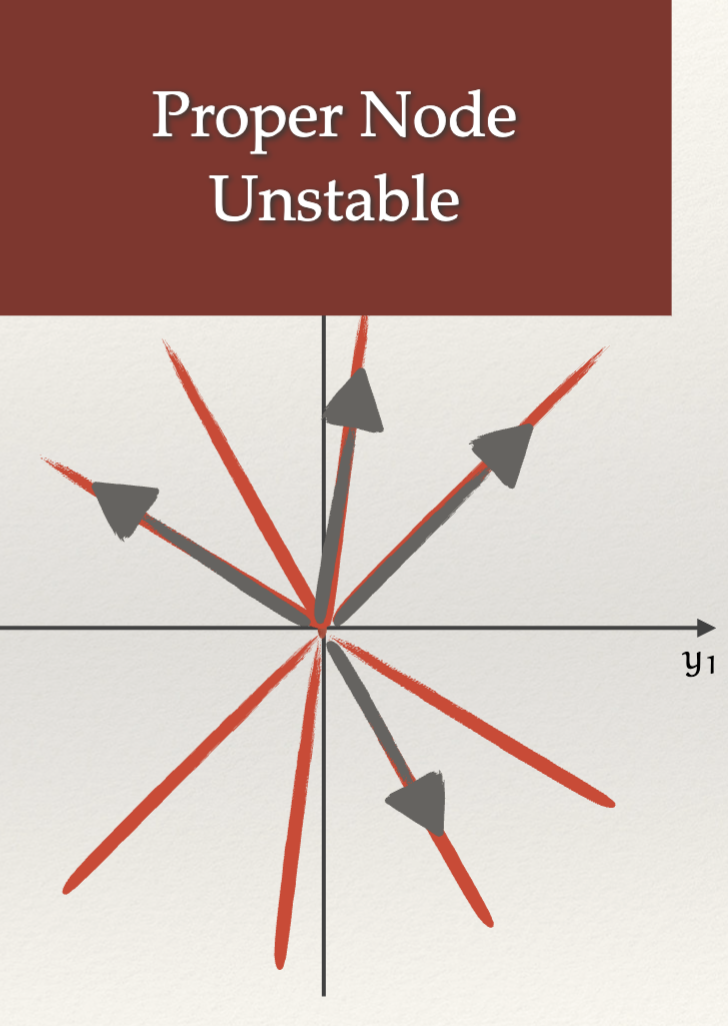
\includegraphics[width=0.15\textwidth]{fig/fig1}}
		\subfigure[$\lambda<0$]{\label{fig2}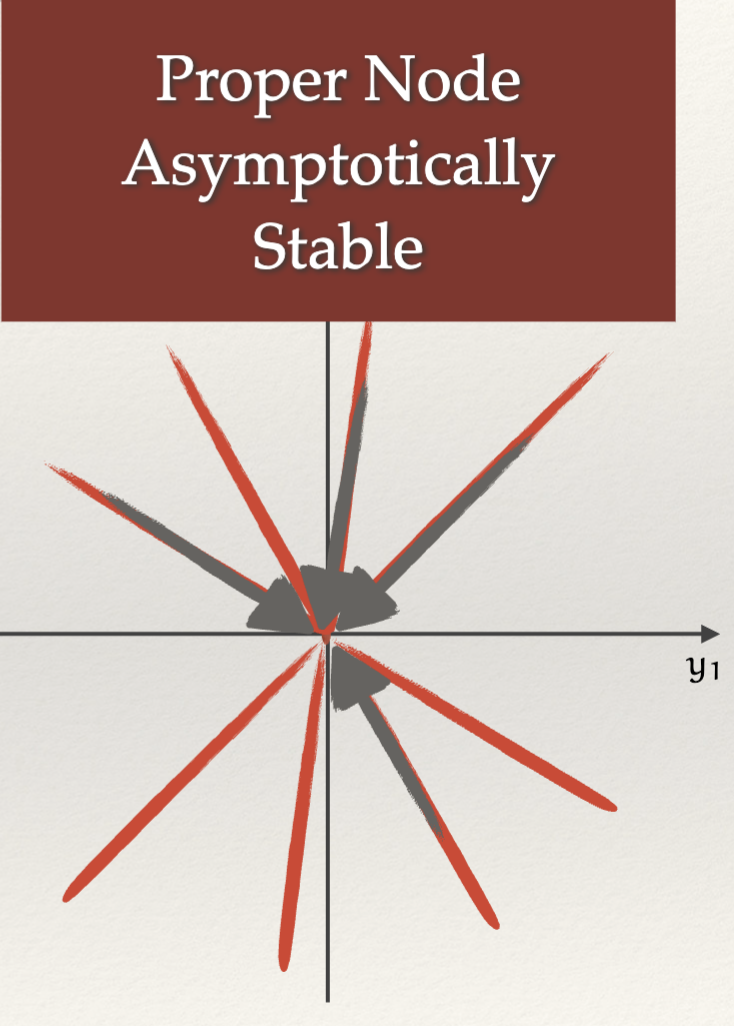
\includegraphics[width=0.15\textwidth]{fig/fig2}}
		\end{figure}
		\item Suppose $\lambda_2>\lambda_1\neq0$. Then, $y=c_1x_1e^{\lambda_1t}+c_2x_2e^{\lambda_2t}$. Let $L_1$ be the line parallel to $x_1$ and $L_2$ be the line parallel to $x_2$.
		\begin{enumerate}
			\item If $c_2=0$, then $y=c_1x_2e^{\lambda_1t}$. If $c_1\neq0$, the trajectory is a half-line of $L_1$. If $\lambda_1>0$, motion is away from the origin. If $\lambda_1<0$, motion is towards the origin. 
			\begin{figure}[H]\centering
			\subfigure[$c_2=0; \lambda_1>0$]{\label{fig3}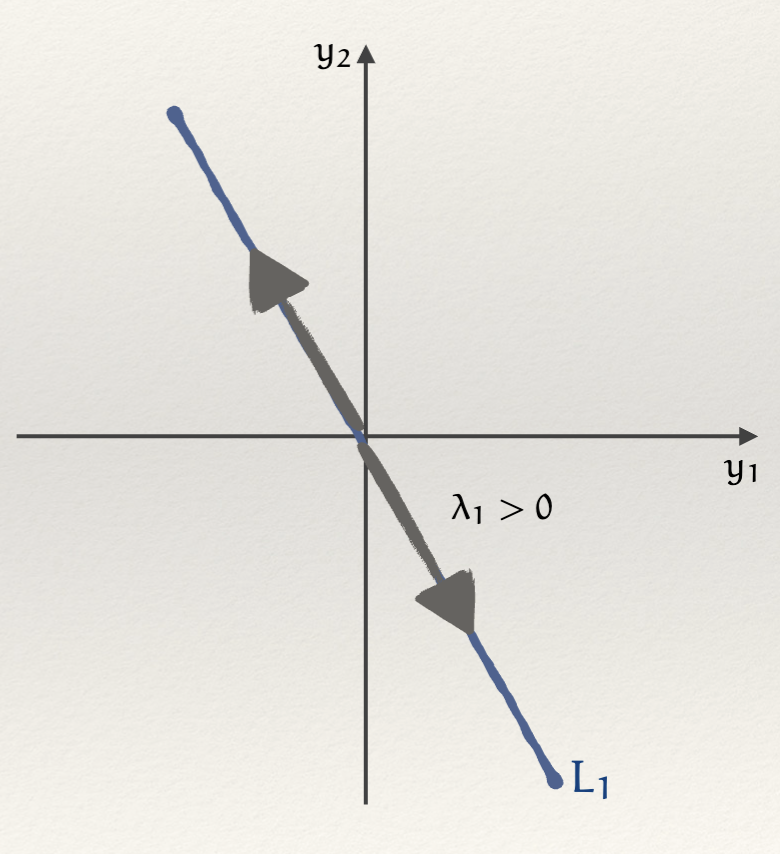
\includegraphics[width=0.2\textwidth]{fig/fig3}}
			\hfill
			\subfigure[$c_2=0; \lambda_1<0$]{\label{fig4}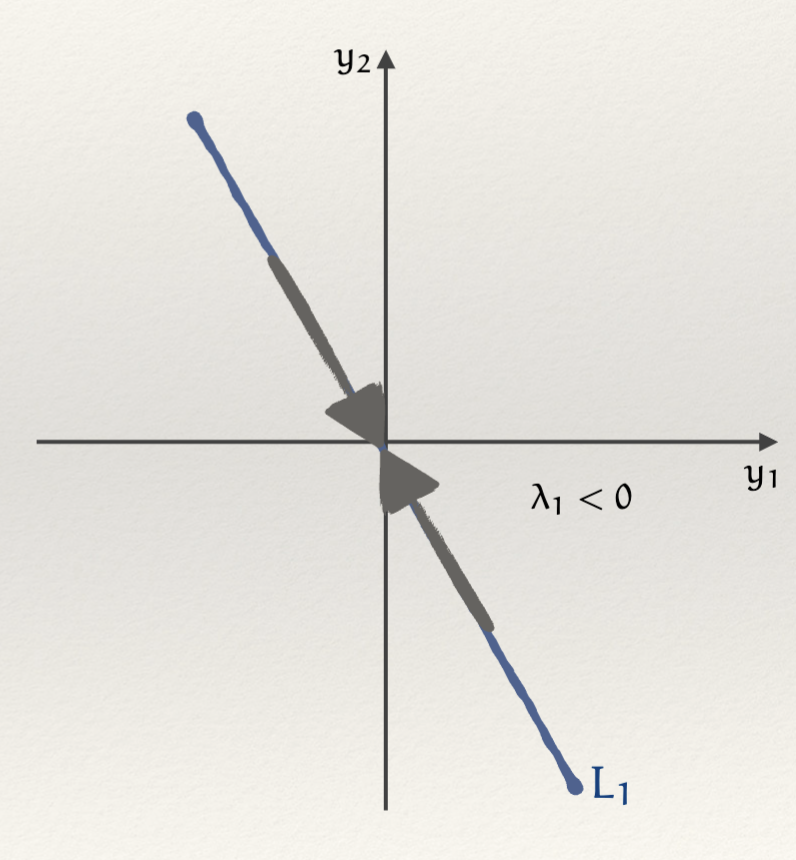
\includegraphics[width=0.2\textwidth]{fig/fig4}}
			\hfill
			\subfigure[$c_1=0; \lambda_2>0$]{\label{fig5}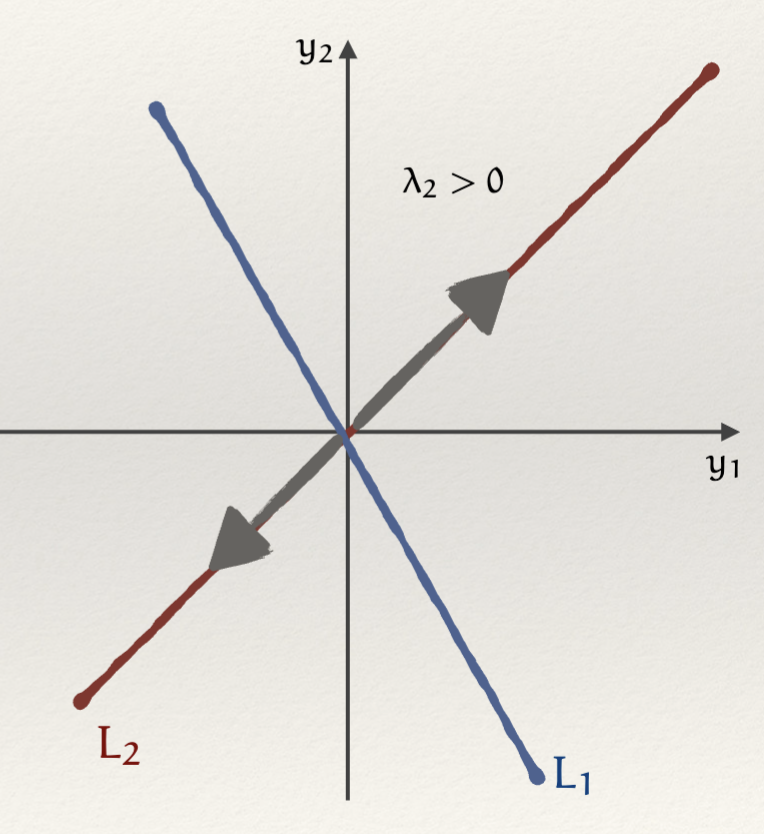
\includegraphics[width=0.2\textwidth]{fig/fig5}}
			\hfill
			\subfigure[$c_1=0; \lambda_2<0$]{\label{fig6}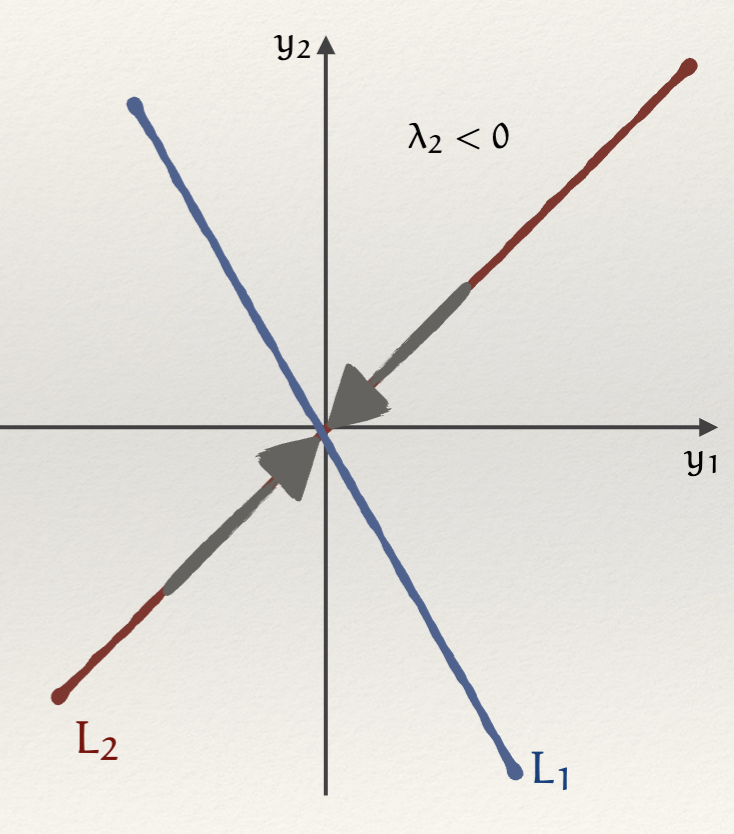
\includegraphics[width=0.2\textwidth]{fig/fig6}}
			\end{figure}
			\item If $c_1=0$, then $y=c_2x_2e^{\lambda_2t}$. If $c_2\neq0$, the trajectory is a half-line of $L_2$. If $\lambda_2>0$, motion moves away from origin. If $\lambda_2<0$, motion moves towards origin.
			\item If $c_1\neq0$ and $c_2\neq0$, then $y=c_1x_1e^{\lambda_1t}+c_2x_2e^{\lambda_2t}$. The trajectory cannot intersect $L_1$ or $L_2$. The trajectories lie entirely in one of the open sectors bounded by $L_1$ and $L_2$. The direction is the same as 
				\begin{itemize}
					\item Note that $e^{-\lambda_2t}y(t)=c_1x_1e^{-(\lambda_2-\lambda_1)t}+c_2x_2$. Therefore as $t\to\infty$, we have $e^{-\lambda_2t}y(t)\to c_2x_2\implies$ trajectory is asymptotically parallel to $L_2$.
					\item Note that $e^{-\lambda_1t}y(t)=c_1x_1+c_2x_2e^{(\lambda_2-\lambda_1)t}$. Therefore as $t\to-\infty$, we have $e^{-\lambda_1t}y(t)\to c_1x_1\implies$ trajectory is asymptotically parallel to $L_1$.
				\end{itemize}
				\begin{enumerate}
					\item If $\lambda_2>\lambda_1>0$. 
					\begin{figure}[H]
						\centering
						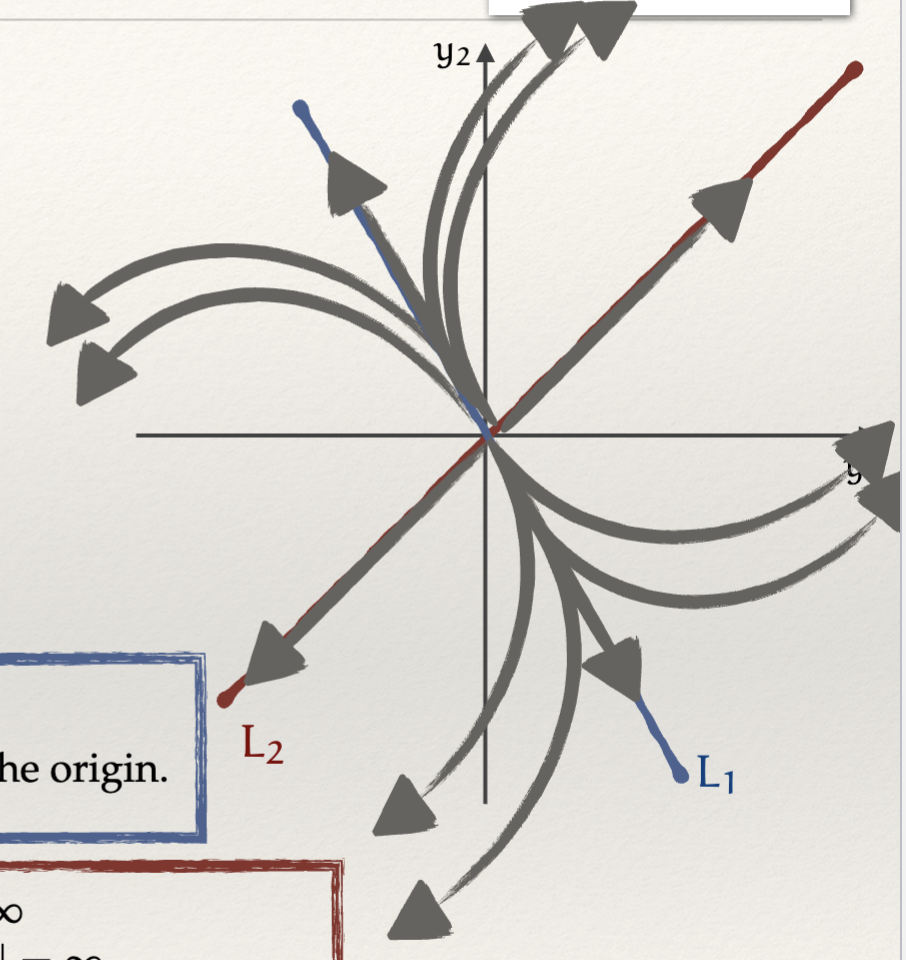
\includegraphics[width=0.38\textwidth]{fig/fig7}\label{fig7}
						\caption{Origin: Unstable Node (Source)}
					\end{figure}
					Note that $\dsst\lim_{t\to-\infty}\|y(t)\|=\lim_{t\to-\infty}\|c_1x_1e^{\lambda_1t}+c_2x_2e^{\lambda_2t}\|=0$. Therefore, the trajectory is asymptotically tangent to $L_1$ at origin. \par 
					Further note $\dsst\lim_{t\to+\infty}\|y(t)\|=\lim_{t\to+\infty}\|c_1x_1e^{\lambda_1t}+c_2x_2e^{\lambda_2t}\|=\infty$, and we know that $\dsst\lim_{t\to\infty}\|y(t)-c_2x_2e^{\lambda_2t}\|=\lim_{t\to\infty}\|c_1x_2e^{\lambda_1t}\|=\infty$. Then, the trajectory is asymptotically parallel to $L_2$, but not tangent to $L_2$.\par 
					\textbf{Direction: Away from the origin. }
					\item If $0>\lambda_2>\lambda_1$. 
					\begin{figure}[H]
						\centering
						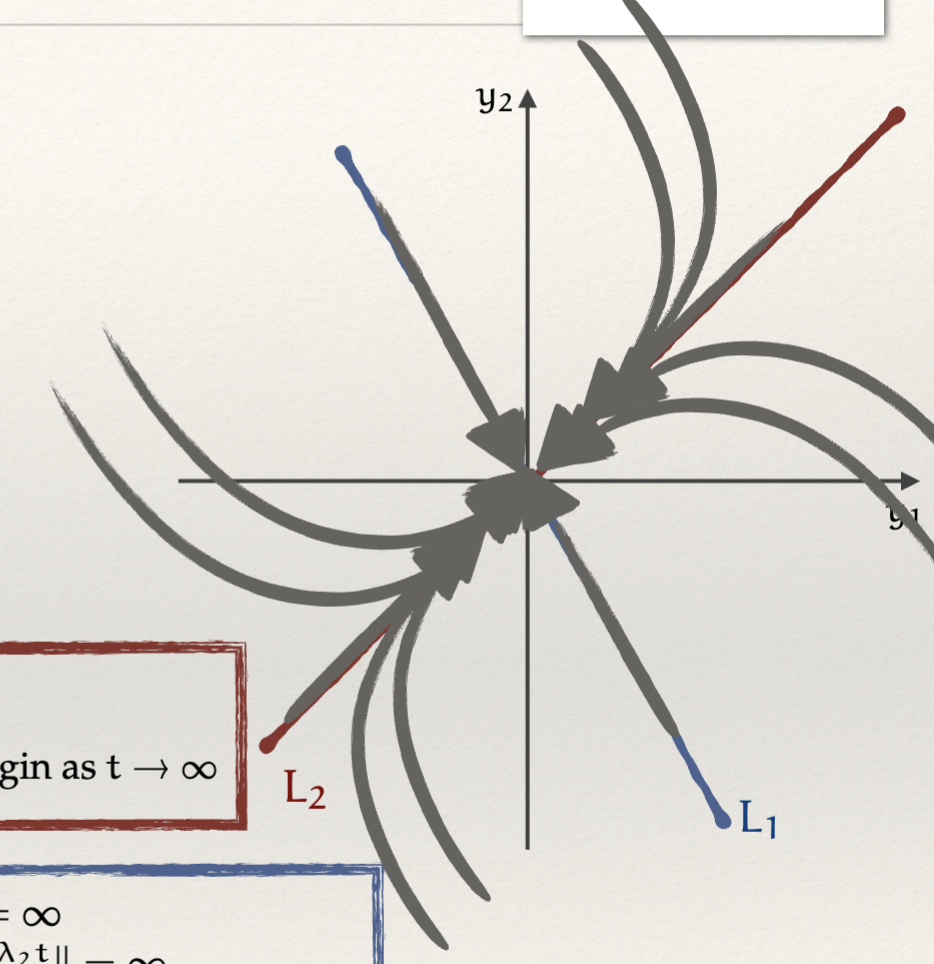
\includegraphics[width=0.38\textwidth]{fig/fig8}\label{fig8}
						\caption{Origin: Asymptotically Stable Node (Sink)}
					\end{figure}
					We have $\dsst\lim_{t\to\infty}\|y(t)\|=\lim_{t\to\infty}\|c_1x_2e^{\lambda_1t}+c_2x_2e^{\lambda_2t}\|=0$, so the trajectory is asymptotically to $L_2$.\par 
					Further we have $\dsst\lim_{t\to-\infty}\|y(t)\|=\lim_{t\to-\infty}\|c_1x_1e^{\lambda_1t}+c_2x_2e^{\lambda_2t}\|=\infty$, and we have that $\dsst\lim_{t\to-\infty}\|y(t)-c_1x_1e^{\lambda_1t}\|=\lim_{t\to-\infty}\|c_2x_2e^{\lambda_2t}\|=\infty$. So, the trajectory is asymptotically parallel to $L_1$.\par 
					\textbf{Direction: Toward the origin.}
					\item If $\lambda_2>0>\lambda_1$
					\begin{figure}[H]
						\centering
						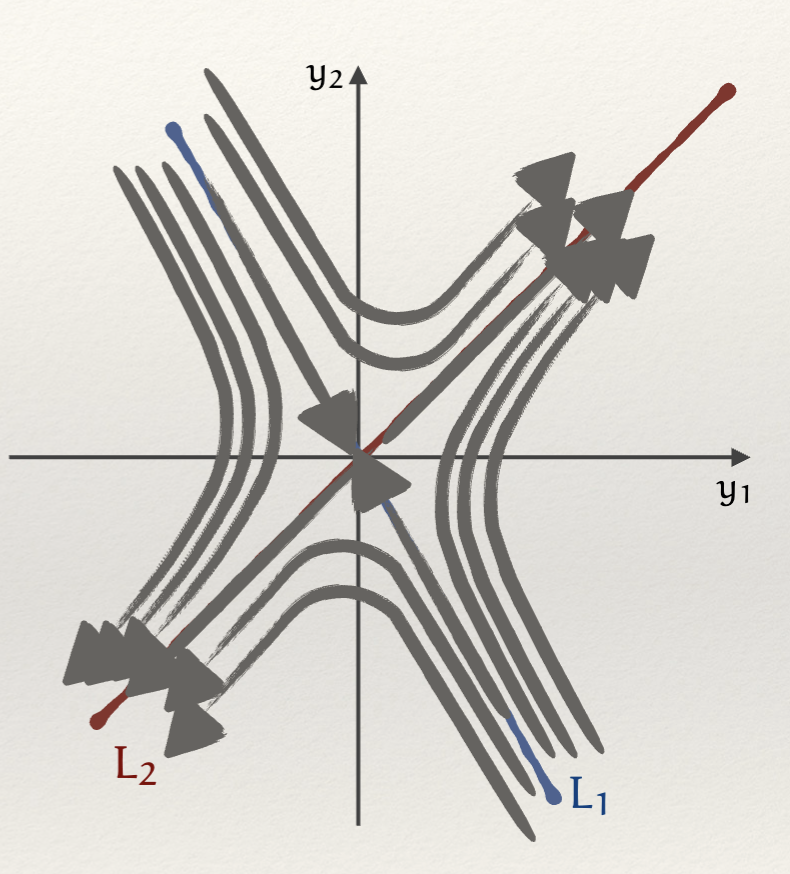
\includegraphics[width=0.38\textwidth]{fig/fig9}\label{fig9}
						\caption{Origin: Unstable Node (Saddle Point)}
					\end{figure}
					Note that $\dsst\lim_{t\to\infty}\|y(t)\|=\lim_{t\to\infty}\|c_1x_1e^{\lambda_1t}+c_2x_2e^{\lambda_2t}\|=\infty$, and we know that $\dsst\lim_{t\to\infty}\|y(t)-c_2x_2e^{\lambda_2t}\|=\lim_{t\to\infty}\|c_1x_1e^{\lambda_1t}\|=0$. Therefore, the trajectory is asymptotically tangent to $L_2$. \par 
					Further we have that $\dsst\lim_{t\to-\infty}\|y(t)\|=\lim_{t\to-\infty}\|c_1x_1e^{\lambda_1t}+c_2x_2e^{\lambda_2t}\|=\infty$, and we know $\dsst\lim_{t\to-\infty}\|y(t)-c_1x_1e^{\lambda_1t}\|=\lim_{t\to-\infty}\|c_2x_2e^{\lambda_2t}\|=0$. Therefore, the trajectory is asymptotically tangent to $L_1$.
					\item If $\lambda_2=0, \lambda_1\neq0$. Then, $y=c_1x_2e^{\lambda_1t}+c_2x_2$. \par $y=c_2x_2$ is a constant solution (a line). 
					\begin{figure}[H]\centering
					\subfigure[$\lambda_1>0$]{\label{fig10}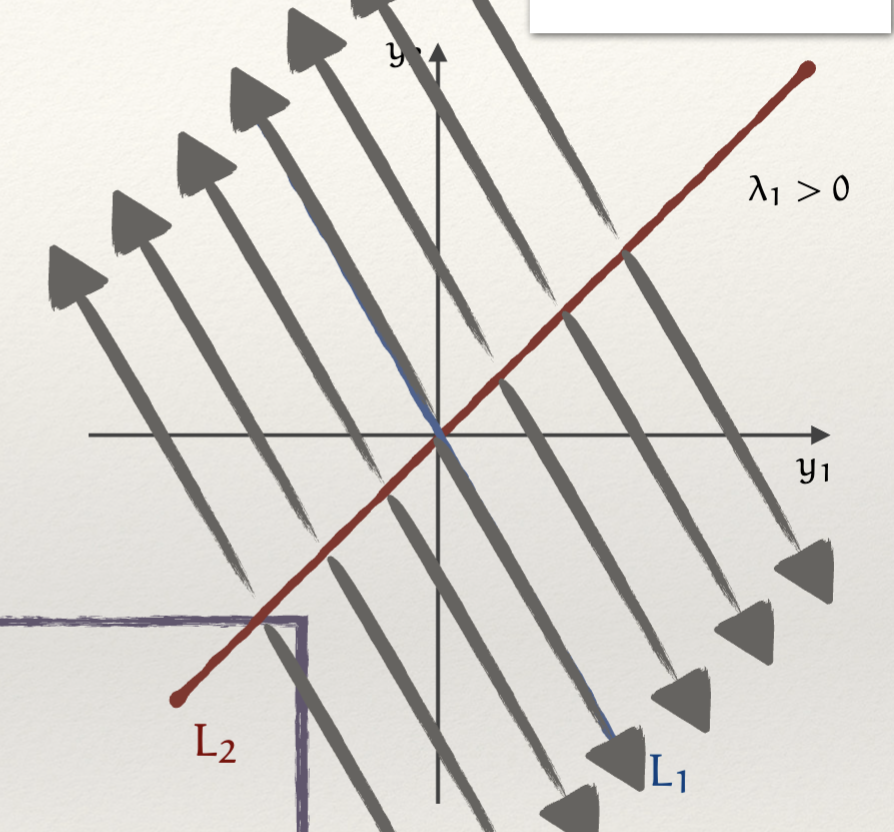
\includegraphics[width=0.38\textwidth]{fig/fig10} }\hfill
					\subfigure[$\lambda_1<0$]{\label{fig11}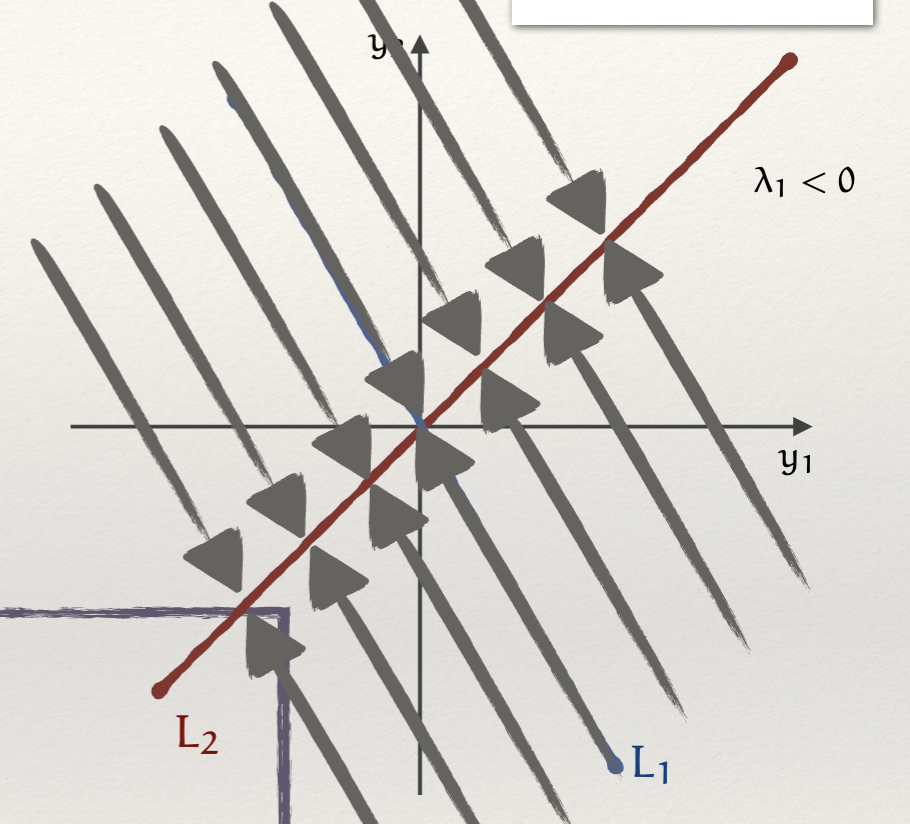
\includegraphics[width=0.38\textwidth]{fig/fig11}}
					\end{figure}
					If $\lambda_1>0$, we have $\dsst\lim_{t\to\infty}\|y(t)\|=\lim_{t\to\infty}\|c_1x_1e^{\lambda_1t}+c_2x_2\|=\infty$.\par 
					If $\lambda_1<0$, we have $\dsst\lim_{t\to\infty}\|y(t)\|=\lim_{t\to\infty}\|c_1x_1e^{\lambda_1t}+c_2x_2\|=0$.\par 
					Also, we know $\dsst\lim_{t\to\infty}\|y(t)-c_1x_1e^{\lambda_1t}\|=\lim_{t\to\infty}\|c_2x_2\|=c_2x_2$.\par 
					We get parallel half-lines because we know all the solutions must be parallel to $L_1$.
				\end{enumerate}
		\end{enumerate}
	\end{enumerate}
	\item Case of Repeated Eigenvalues (Defective): \[y=c_1xe^{\lambda t}+c_2e^{\lambda t}(w+tx).\]
	\begin{enumerate}
		\item Assume $\lambda\neq0$. Call $L$ the line through origin parallel to $x$. If $c_2\neq0$, the solution is a parametric equation of the half-line of $L$. 
		\begin{itemize}
			\item In the direction of $x$ if $c_1>0$.
			\item In the direction of $-x$ if $c_1<0$.
		\end{itemize}
		\item Assume $c_2\neq0$.\par 
		The trajectory cannot intersect $L$ since every point on $L$ is on a trajectory obtained by setting $c_2=0$. The trajectory must lie entirely in on of the open half-planes bounded by $L$, but does not obtain any point on $L$. Since the initial point $\qty(y_1(0),y_2(0))$ defined by $y(0)=c_1x+c_2w$ is on the trajectory, we can determine which half-plane contains the trajectory from the sign of $c_2$.\par 
		We call the half-plane where $c_2>0$ the positive half-plane and $c_2<0$ the negative half-plane. \par 
		Multiply the solution by $e^{-\lambda t}$, we have \[e^{-\lambda t}y(t)=c_1x+c_2w+c_2tx.\] When $\qty|t|$ is large, the last term is dominant; therefore, 
		\begin{enumerate}
			\item Along the trajectories in the positive half-plane: \par 
			The direction of $y(t)$ approaches $x$ as $t\to+\infty$; the direction of $y(t)$ approaches $-x$ as $t\to-\infty$.
			\item Along the trajectories in the negative half-plane:\par 
			The direction of $y(t)$ approaches $-x$ as $t\to+\infty$; the direction of $y(t)$ approaches $x$ as $t\to-\infty$.
		\end{enumerate}
		\item If $\lambda>0$: \[\lim_{t\to\infty}\|axe^{\lambda t}+c_2e^{\lambda t}(w+tx)\|=\infty\] and \[\lim_{t\to-\infty}\|c_1xe^{\lambda t}+c_2e^{\lambda t}(w+tx)\|=0.\]
		\begin{figure}[H]
			\centering
			\subfigure[$\lambda>0$: Origin: Improper Node (Undable)]{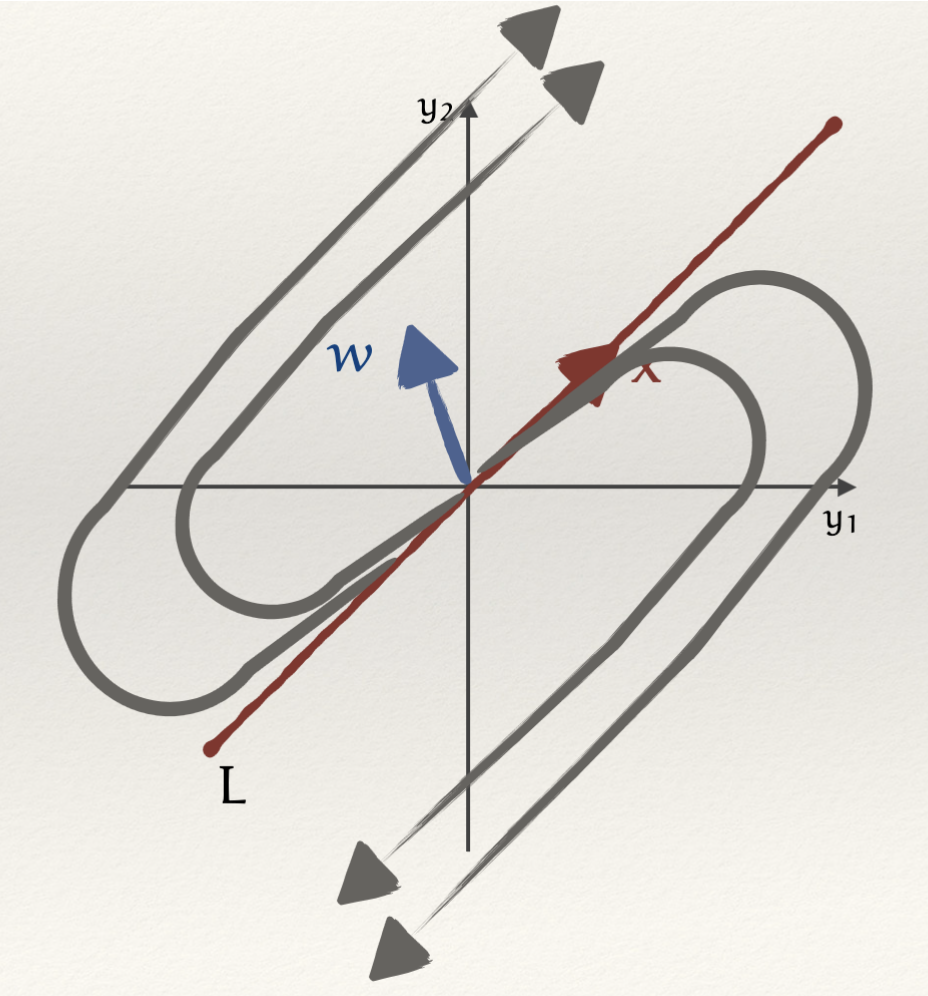
\includegraphics[width=0.38\textwidth]{fig/fig12}\label{fig12}}
			\hfill
			\subfigure[$\lambda<0$: Origin: Improper Node (Asymptotically Stable)]{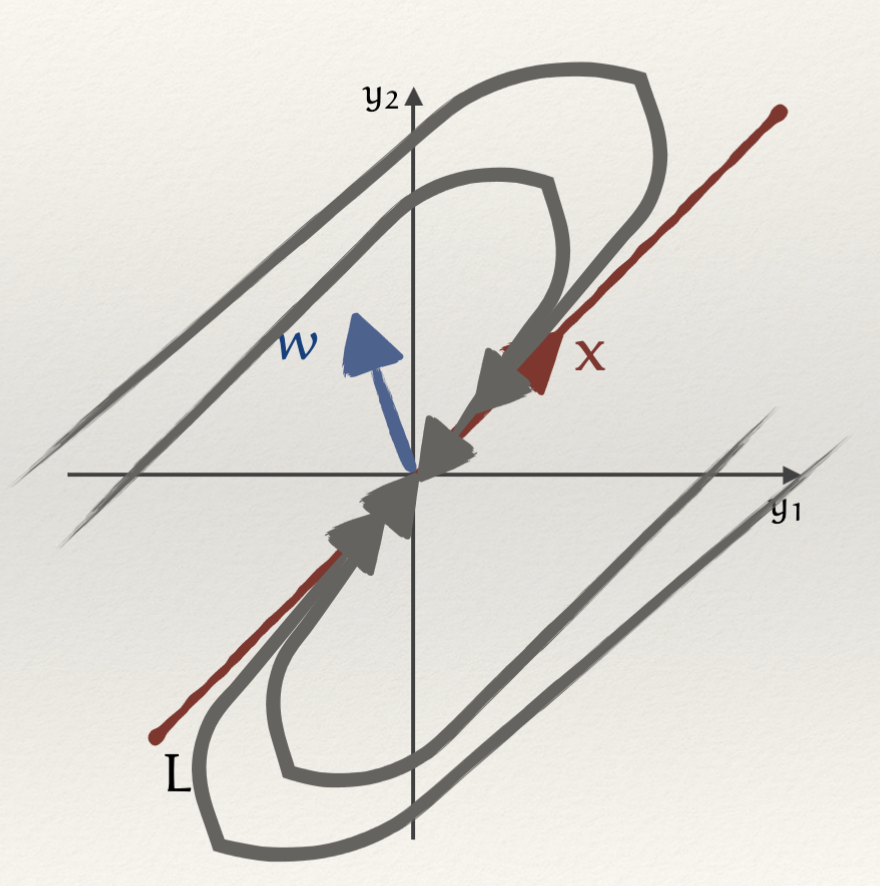
\includegraphics[width=0.38\textwidth]{fig/fig13}\label{fig13}}
		\end{figure}
		\item If $\lambda<0$: \[\lim_{t\to+\infty}\|c_1xe^{\lambda t}+c_2e^{\lambda t}(w+tx)\|=0\] and \[\lim_{t\to-\infty}\|c_1xe^{\lambda t}+c_2e^{\lambda t}(w+tx)\|=\infty\]
	\end{enumerate}
	\item Case of Complex Eigenvalues: \[y=e^{\alpha t}[c_1(\cos(\beta t)u-\sin(\beta t)v)+c_2(\cos(\beta t)v+\sin(\beta t)u)],\] which can be written as \[y=e^{\lambda t}\qty{[c_1\cos(\beta t)+c_2\sin(\beta t)]u+[-c_1\sin(\beta t)+c_2\cos(\beta t)]v}.\] Call $U=\dfrac{u}{\|u\|}$ and $V=\dfrac{v}{\|v\|}$, and multiply the solution by $e^{-\lambda t}$, and call the curve traversed by $e^{-\alpha t}y$ a \textit{shadow trajectory}, then \[e^{-\alpha t}y=z_1U+z_2V,\] where $z_1=\|u\|[c_1\cos(\beta t)+c_2\sin(\beta t)]$ and $z_2=\|v\|[-c_1\sin(\beta t)+c_2\cos(\beta t)]$. We can verify that $\dfrac{z_1^2}{\|u\|^2}+\dfrac{z_2^2}{\|v\|^2}=c_1^2+c_2^2$, meaning the shadow trajectories are ellipses centered at the origin with axes parallel to $U$ and $V$. 
	\begin{figure}[H]\centering
		\subfigure[$\alpha=0$: Origin: Center (Stable)]{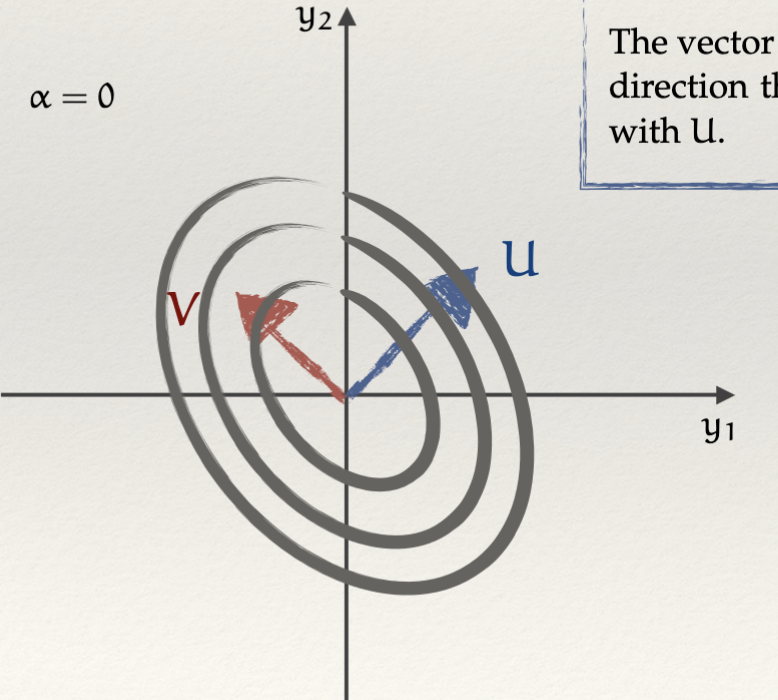
\includegraphics[width=0.3\textwidth]{fig/fig14}}\label{fig14}
		\subfigure[$\alpha>0$: Origin: Spiral Point (Unstable)]{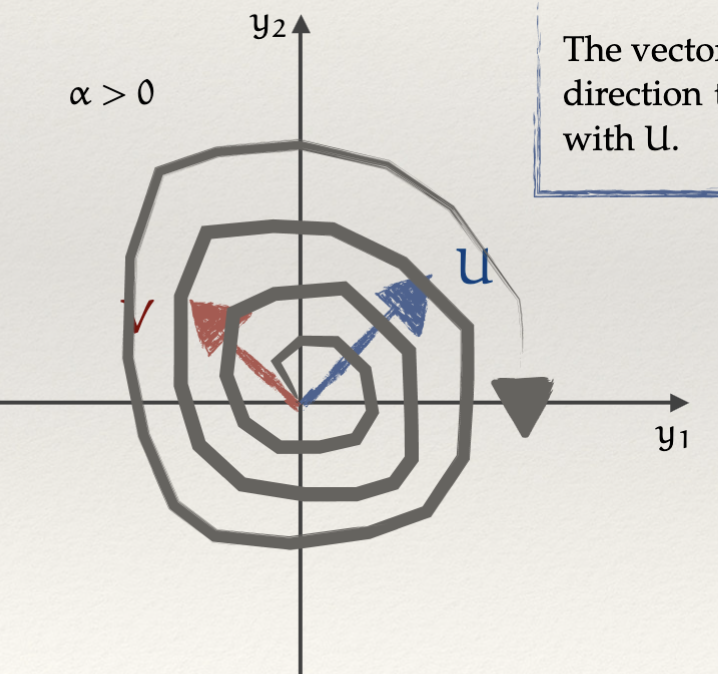
\includegraphics[width=0.3\textwidth]{fig/fig15}}\label{fig15}
		\subfigure[$\alpha<0$: Origin: Spiral Point (Unstable)]{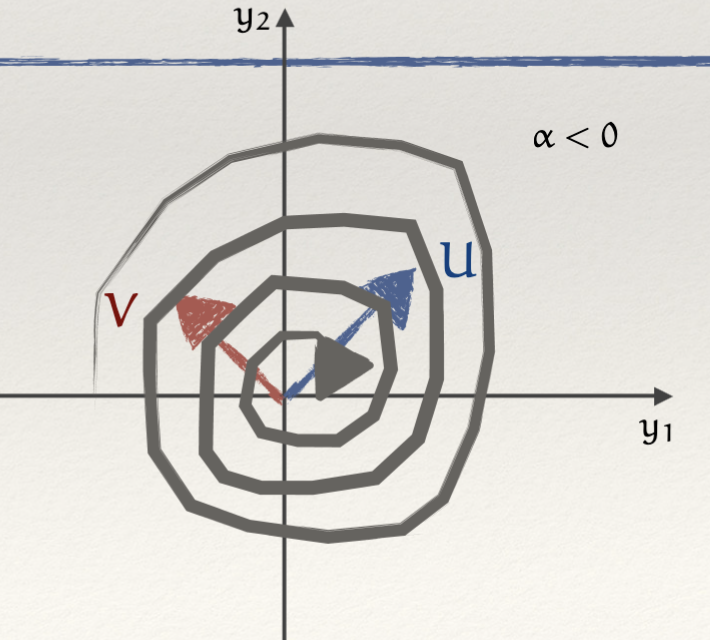
\includegraphics[width=0.3\textwidth]{fig/fig16}}\label{fig15}
	\end{figure}
\end{itemize}

\subsection{Autonomous System of Differential Equations}
\subsubsection{The Predator-Prey Model}
\begin{enumerate}
	\item Setting-ups and Assumptions: 
	\begin{enumerate}
		\item Rabbits: $R(t)=$ the number of rabbits. \par The rabbits have ample food supplies.\par In the absence of predators, the food supply would support exponential growth of the prey: \[\dv{R}{t}=rR,\quad r>0.\]
		\item Wolves: $W(t)=$ the number of wolves. \par The wolves feed on the rabbits. In the absence of prey, the predators would decline at a rate which is proportional the actual population: \[\dv{W}{t}=-kW,\quad k>0.\]
	\end{enumerate}
	\begin{thm}{Principle of Mass Action}
	Given two populations, the rate of contact between the populations is proportional to the product of their sizes.
 	\end{thm}
 	\item In the model, we need to consider: (a) the cause of death for the prey are the predators; and (b) the birth rate of the predators depends on the prey. So, we have the following system of ODEs: \[\begin{cases}\dsst\dv{R}{t}=rR-aRW\\\\\dsst\dv{W}{t}=-kW+bRW\end{cases},\quad k,r,a,b>0.\]
 	\item \begin{df}{Autonomous Systems of ODEs}\[\begin{cases}x'(t)=f(x,y),\quad x=x(t),\ population\ of\ x\ at\ time \ t\\y'(t)=g(x,y), \quad y=y(t),\ population\ of\ y\ at\ time \ t\end{cases}\]\end{df}
 	\item \begin{df}{Nullclines} Given $\begin{cases}x'=f(x,y)\\y'=g(x,y)\end{cases}$, the \textit{$x$-nullclines} are the curves in the $xy$-plane that satisfy $f(x,y)=0$. Along these curves, we have $x'=0$. The \textit{$y$-nullclines} are the curves in the $xy$-plane that satisfy $g(x,y)=0$. Along these curves, we have $y'=0$.\end{df}
 	\item \begin{df}{Equilibrium Point}Any point at which an $x$-nullicline intersects a $y$-nullcline is an \textit{equilibrium point}, where both $x$ and $y$ are not changing. \end{df}
\end{enumerate}
\begin{thm}{Phase-Plane Analysis}
\begin{enumerate}
	\item Set $f(x,y)$ and $g(x,y)$ to $0$ to find the nullclines and the equilibrium points.
	\item Draw nullclines and equilibria on the $xy$-plane.
	\item Study the signs of functions $f$ and $g$, and draw the combined arrows in each different region of the plane. \textit{At which values of $x$ and $y$ are functions $f$ and $g$ increasing or decreasing? }
	\item Describe the equilibrium points (extinction of both $x$ and $y$, extinction of $x$ or $y$, coexistence of $x$ and $y$, etc.)
	\item Estimate the behavior of $x(t)$ and $y(t)$ as $t\to\infty$, and make conclusion about the long term behavior of the populations.
\end{enumerate}
\end{thm}
\begin{eg}
	Consider \[\begin{cases}R'=rR-aRW\\W'=-kW+bRW\end{cases},\quad k,r,a,b>0.\]
	\begin{enumerate}
		\item Find $R$-nullclines: $R'=rR-aRW=R(r-aW)=0\implies R=0\text{ or }W=\dfrac{r}{a}.$
		\item Find $W$-nullclines: $W'=-kW+bRW=W(bR-k)=0\implies W=0\text{ or }R=\dfrac{k}{b}$
		\item Find equilibrium points: $E_1(0,0)$ and $E_2\qty(\dfrac{k}{b},\dfrac{r}{a})$.
		\item Study sign of $R'$: $R'<0\implies rR-aRW>0\implies R>0\text{ and }W<\dfrac{r}{a}$.
		\item Study sign of $W'$: $W'>0\implies -kW+bRW>0\implies W>0\text{ and }R>\dfrac{k}{b}$.
	\end{enumerate}
\end{eg}

\subsubsection{Competing Species}
Let $x,y$ be populations of two species $X, Y$. we model $x,y$ using logistic growth: \[x'=rx\qty(1-\dfrac{x}{K}),\quad y'=sy\qty(1-\dfrac{y}{L}),\quad r,K,s,L>0\]
\begin{eg}
	Model I \[x'=0.05x\qty(1-\dfrac{x}{20})-0.002xy\quad y'=0.09\qty(1-\dfrac{y}{15})-0.15xy\]	
\end{eg}
\begin{eg}
	Model II \[x'=x(0.2-0.05x-0.02y)\quad y'=y(0.1-0.01x-0.02y)\]	
\end{eg}
\begin{eg}
	Model III \[x'=6x-(2/3)x^2-xy\quad y'=10y-y^2-2xy\]	
\end{eg}

\subsubsection{SIR Model}
\begin{eg}
	The SIR Model\par 
	Let $S$ be the number of the \textit{susceptible}, the people who are not yet sick but who could become sick, $I$ the number of the \textit{infected}, the people who are currently sick, and $R$ the number of \textit{recovered}, the people who have been sick and can no longer infect others or be reinfected.\par 
	Since $S+I+R=n$, the total population, we only need the populations of $S$ and $I$, and then we can compute $R$. Therefore, we form the following system of equations: 
	\[\dsst\dv{S}{t}=-aSI\quad \dv{I}{t}=aSI-bI\]
	Using the phase plane analysis, we can find a threshold value $S_T$ such that it will maximize $I$. Considering the multi-variable chain rule: \[\dv{I}{S}=\dv{I}{t}\dv{t}{S}=\dfrac{aSI-bI}{-aSI}=-1+\dfrac{b}{aS}\] Then, we can solve for $I$ as a function of $S$ by separation of variables: \[I(S)=-S+\dfrac{b}{a}\ln(S)+C.\] Given some initial conditions, we can easily find $C$. By substituting different values of $S$ we can find the value of $I$ at any desired time. 
\end{eg}


\newpage
\section{Second Order ODEs}
\end{document}